% Interim report (Polish). Build: see docs/report/README.md.
\documentclass[11pt,a4paper]{article}

% Collective course-project byline.
\newcommand{\zespol}{Zespół projektu, AGH}

\usepackage{fontspec}
\setmainfont{lmroman10-regular.otf}[
  BoldFont=lmroman10-bold.otf,
  ItalicFont=lmroman10-italic.otf,
  BoldItalicFont=lmroman10-bolditalic.otf]
\setsansfont{lmsans10-regular.otf}[BoldFont=lmsans10-bold.otf]
\setmonofont{lmmono10-regular.otf}
\usepackage[polish]{babel}
\usepackage[margin=2.5cm]{geometry}
\usepackage{amsmath,amssymb}
\usepackage{graphicx}
\usepackage{booktabs,tabularx,array,makecell}
\usepackage[font=small,labelfont=bf,labelsep=period,justification=raggedright,singlelinecheck=true]{caption}
\usepackage{enumitem}
\usepackage{xcolor}
\usepackage{tikz}
\usetikzlibrary{positioning,arrows.meta,fit,backgrounds,babel}
\usepackage{placeins}
\usepackage[numbers,sort&compress]{natbib}
\setlength{\bibsep}{2pt}
\usepackage[colorlinks=true,linkcolor=blue!50!black,citecolor=blue!50!black,urlcolor=blue!50!black]{hyperref}

\graphicspath{{../figures/}}
\setlist{itemsep=2pt,topsep=4pt}
\emergencystretch=3em
\renewcommand{\arraystretch}{1.2}
% note under a table: what the caption would otherwise have to explain
\newcommand{\tablenote}[1]{\par\vspace{4pt}{\footnotesize\raggedright #1\par}}
\newcolumntype{Y}{>{\raggedright\arraybackslash}X}
\newcommand{\code}[1]{\texttt{#1}}
\newcommand{\cell}[1]{\textit{#1}}

\newcommand{\questionOne}{Czy to, że część inwestorów wycenia spółki przez ceny ich dostawców, przyspiesza reakcję rynku na szok
surowcowy, czy przesuwa ją na kolejne sesje?}
\newcommand{\questionTwo}{Jak skład strategii inwestorów i~siła naśladowania zmieniają wahania cen i~tempo ich dostosowania?}
\newcommand{\questionThree}{Czy wspólny portfel inwestora (limit ryzyka, rebalansowanie) sprawia, że razem poruszają się spółki, których
graf nie łączy?}

\title{Opóźniona reakcja cen akcji na zmiany cen surowców w~agentowym modelu wieloaktywowym}
\author{\zespol}
\date{26 listopada 2026}
\begin{document}
\maketitle
\begin{abstract}
Badamy, jak sposób wyceny spółek wpływa na czas reakcji ich cen na dzienne zmiany cen surowców.
W~modelu 18 amerykańskich spółek inwestorzy handlują w~oddzielnych arkuszach zleceń. Część z~nich obserwuje ceny surowców i~indeksu,
a~część wykorzystuje dodatkowo ceny akcji dostawców na symulowanym rynku.
W~690 przebiegach na jednej historii lat 2024--2025 porównujemy warianty na wspólnych ziarnach losowych.
Przy zastąpieniu 250 z~300 wyceniających agentami sieciowymi reakcja dwóch rafinerii na zmianę ich wyceny
referencyjnej osłabła w~tej samej sesji, a~wzrosła w~następnej i~w~obu sesjach łącznie. Współczynnik reakcji
w~następnej sesji wzrósł o~0,515 (95\% przedział bootstrapowy [0,480; 0,550]).
Skład z~większym udziałem inwestorów trendowych i~silniejsze naśladowanie zwiększyły odchylenia cen od wyceny
referencyjnej. Wyłączenie limitu ryzyka i~rebalansowania nie dało wyraźnego spadku współruchu spółek niepowiązanych.
Poza okresem estymacji wag zarówno pełny graf, jak i~same bezpośrednie ekspozycje na surowce i~indeks
dały medianę korelacji z~rzeczywistymi stopami zwrotu równą 0,595. W~danych z~lat 2024--2025 test stóp
zwrotu wzdłuż krawędzi grafu nie wykrył jednodniowego opóźnienia widocznego w~symulacji.
\par\medskip\noindent\textbf{Słowa kluczowe:} model agentowy, arkusz zleceń, dyfuzja informacji, ceny surowców, współruch akcji.
\end{abstract}

\section{Wprowadzenie}\label{sec:wprowadzenie}
Dwie rafinerie mogą mieć podobną ekspozycję na ropę, choć inwestorzy dochodzą do ich wyceny różnymi drogami.
Jeden obserwuje bezpośrednio WTI. Drugi obserwuje również kurs spółki wydobywczej, który sam musi najpierw
zareagować na zmianę ceny surowca. Czy uwzględnienie tej dodatkowej informacji przyspiesza reakcję rynku,
czy przenosi część dostosowania na kolejną sesję? Porównujemy te reguły na tej samej historii cen zewnętrznych
i~przy identycznej konstrukcji giełdy.

\paragraph{Od informacji do zlecenia.}
W~modelu Chiarelli i~Iori strategie heterogenicznych uczestników wpływają na zmienność, wolumen i~spread poprzez zlecenia
w~arkuszu~\cite{chiarella-iori}. U~Honga i~Steina stopniowa dyfuzja informacji i~handel zgodny z~trendem zmieniają
przebieg reakcji ceny~\cite{hongstein1999}. W~naszym eksperymencie zmieniamy skład strategii i~wagę sygnału społecznego,
a~dostosowanie mierzymy względem jawnej trajektorii referencyjnej. W~przeciwieństwie do wyjściowego modelu jednego aktywa
Skrzyńskiego~\cite{skrzynski} każdy kurs w~sieci może stać się informacją dla inwestorów handlujących inną akcją.

\paragraph{Powiązania gospodarcze i~opóźnienie.}
Cohen i~Frazzini obserwują ujawnione relacje konkretnych firm i~badają późniejsze stopy zwrotu dostawców
po informacjach o~ich klientach, w~horyzoncie miesięcznym~\cite{cohen}.
U~nas relacje między branżami wskazują potencjalne zależności między akcjami. W~głównym przykładzie informacja biegnie
od wydobywcy do rafinerii, a~jednostką czasu jest sesja. Historyczne zmiany WTI mogą mieć różne źródła popytowe
i~podażowe~\cite{kilian2009}. Używamy obserwowanej zmiany jako wejścia do symulacji bez identyfikowania jej przyczyny.
Osobny eksperyment pozwala zadać wiadomość o~jednej spółce w~znanym momencie.

\paragraph{Współruch poza grafem.}
Efekt majątkowy i~sprzedaż aktywów ze wspólnych portfeli mogą przenosić zaburzenia między rynkami~\cite{kyle,caccioli2014}.
Wyłączamy kolejno limit ryzyka i~rebalansowanie, a~następnie mierzymy współruch pozostały po uwzględnieniu wspólnej informacji.
\paragraph{Pytania badawcze.} Stawiamy trzy pytania i~dla każdego formułujemy hipotezę ocenianą według reguły
zapisanej przed badaniem głównym (rozdz.~\ref{sec:statystyka}).
\begin{enumerate}[label=\textbf{P\arabic*.}, leftmargin=2.2em]
  \item \questionOne{} \emph{H1: więcej takich inwestorów skraca opóźnienie} (eksperyment~E1).
  \item \questionTwo{}
  \emph{H2: więcej strategii trendowych i~silniejsze naśladowanie zwiększają zmienność, odchylenia od trajektorii
  referencyjnej i~spóźnioną reakcję} (eksperyment~E2).
  \item \questionThree{} \emph{H3: wyłączenie tych reguł zmniejsza współruch spółek niepowiązanych} (eksperymenty E3a
  i~E3b).
\end{enumerate}

\section{Dane i~dobór powiązań między spółkami}\label{sec:dane}

\begin{table}[!htbp]
\centering\small
\caption{Dane i~ich rola w~modelu.}\label{tab:dane}
\begin{tabularx}{\textwidth}{@{}Y l Y@{}}
\toprule
Dane & Źródło & Rola \\
\midrule
Ropa WTI, gaz Henry Hub, S\&P~500 (dzienne) & FRED~\cite{data-fred} & sygnały zewnętrzne, zmienna kontrolna \\ \addlinespace[3pt]
Miedź (LME, cena rozliczeniowa, dzienna) & Westmetall~\cite{data-westmetall} & sygnał zewnętrzny \\ \addlinespace[3pt]
Złoto (kontrakty terminowe, dzienne) & Yahoo Finance~\cite{data-yahoo} & sygnał zewnętrzny \\ \addlinespace[3pt]
Ceny i~wolumeny 18 spółek & Yahoo Finance & wagi grafu (2021--2023), ceny startowe (2.01.2024), walidacja
  (2024--2025) \\ \addlinespace[3pt]
Tabele przepływów międzygałęziowych (71 branż) & BEA~\cite{data-bea} & struktura grafu \\ \addlinespace[3pt]
Kody SIC & SEC EDGAR~\cite{data-edgar} & przypisanie spółek do branż \\

\bottomrule
\end{tabularx}
\end{table}

Okres obejmuje 1255 dni sesyjnych 2021--2025. Prawdziwe ceny akcji wchodzą do symulacji tylko jako stan początkowy
z~2 stycznia 2024~r.; w~trakcie przebiegu z~danych historycznych aktualizuje się wyłącznie pięć szeregów zewnętrznych.

Spółki dobrano celowo, aby objąć wydobycie, przetwórstwo, odbiorców surowców i~sektory porównawcze.
Warunkiem była dostępność dziennych cen przez cały okres. Uzasadnienia wyboru dokumentują działalność spółek,
klasyfikację SIC/BEA i~ich ekspozycje z~lat 2021--2023. Wymóg kompletności szeregu obejmował także lata porównania.
Dla każdego dnia, w~którym handlowano akcjami, zestawiliśmy ceny surowców i~wartość indeksu S\&P~500.
Jeśli tego dnia brakowało notowania, przyjmowaliśmy ostatnią znaną wartość danego szeregu, najwyżej przez trzy kolejne sesje.
Dzienne stopy zwrotu akcji obliczyliśmy z~cen uwzględniających podziały akcji i~wypłaty dywidend.
Jako cenę początkową każdej akcji w~symulacji przyjęliśmy jej kurs zamknięcia z~2 stycznia 2024~r.,
skorygowany wyłącznie o~podziały akcji.

Wartość zewnętrzna przypisana do dnia zmienia się na początku
odpowiedniej sesji modelu; agent uzyskuje do niej dostęp zgodnie ze swoim opóźnieniem obserwacji.
To umowna synchronizacja dziennych danych, która nie odwzorowuje godzin publikacji poszczególnych notowań.

Tabele BEA opisują zakupy między branżami. Do oceny wybraliśmy 54 pary spółek, dla których zakupy
od branży dostawcy stanowiły co najmniej 2\% wartości produkcji branży odbiorcy. Następnie sprawdziliśmy,
czy profil działalności obu spółek uzasadnia przeniesienie zależności branżowej na daną parę.
Zachowaliśmy w~ten sposób cztery powiązania wydobywców z~rafineriami, cztery powiązania rafinerii
z~liniami lotniczymi i~dwa z~przewoźnikiem drogowym (rys.~\ref{fig:graf}).
W~pierwszej grupie uzasadnieniem jest zakup ropy do przerobu, w~dwóch pozostałych --- zakup paliwa.
Sam próg obejmował również pary takie jak producenci stali i~aluminium: BEA zalicza ich do jednej branży,
choć wykorzystują inne surowce. Takie pary pominięto. Graf opisuje ekspozycje branżowe bez informacji o~kontraktach poszczególnych firm.

Osobno uwzględniliśmy cztery powiązania producentów układów obliczeniowych z~operatorami centrów danych.
Zakup serwerów jest wydatkiem inwestycyjnym, którego tabela bieżących nakładów nie ujmuje.
Te powiązania przyjęliśmy jako założenie eksperymentu z~wiadomością o~NVDA.

\begin{figure}[!htbp]
\centering
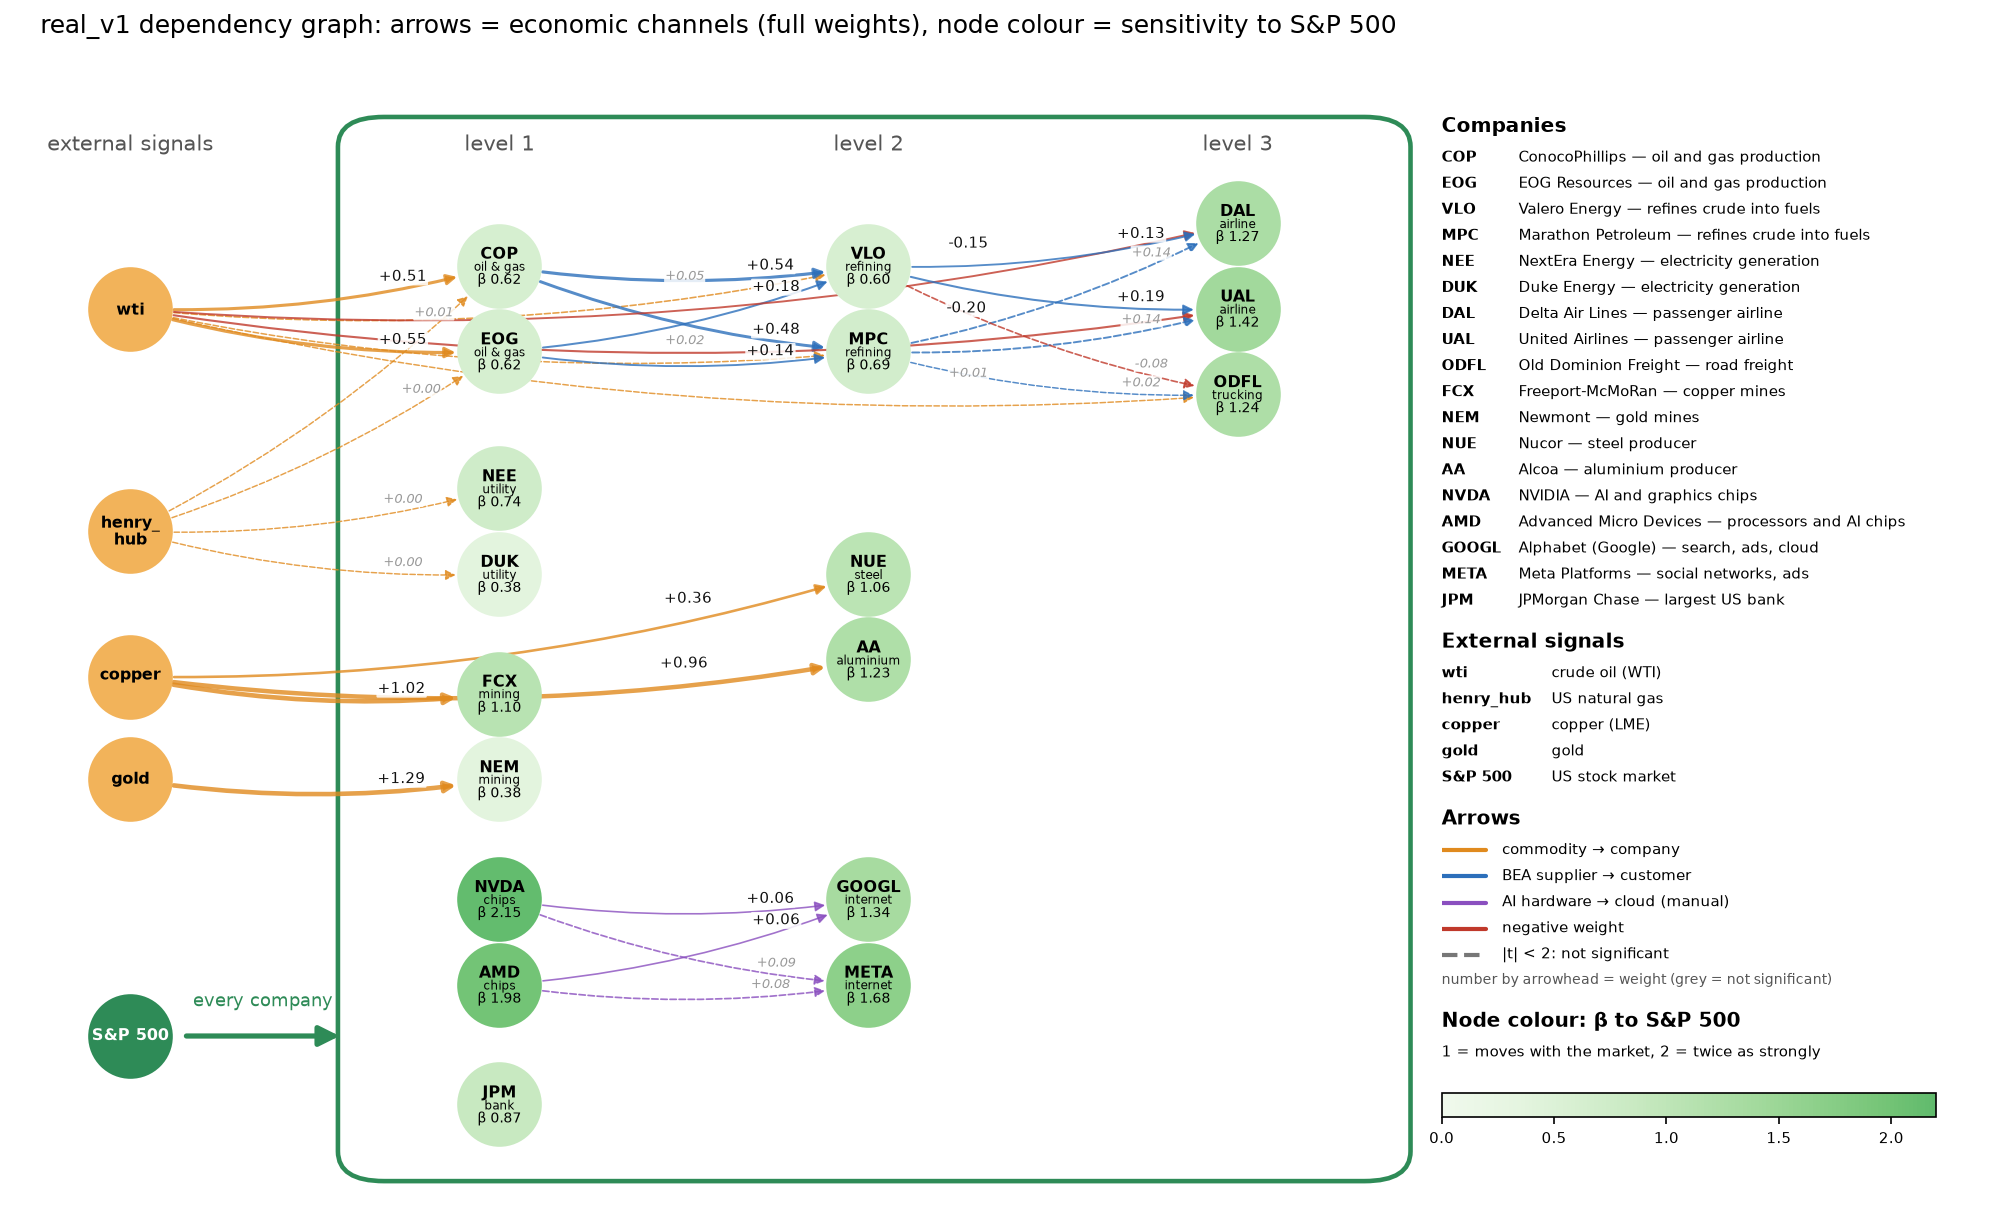
\includegraphics[width=\textwidth,trim=0 0 0 25bp,clip]{f2_graph_real_v1.png}
\caption{Powiązania między sygnałami zewnętrznymi a~spółkami oraz między spółkami. Liczby przy strzałkach oznaczają wagi w~modelu pełnym, a~linie przerywane oznaczają wagi o~$|t|<2$. Jedna zielona strzałka od indeksu S\&P~500 oznacza bezpośrednie powiązanie indeksu z~każdą z~18 spółek. Nasycenie zieleni wskazuje wrażliwość danej spółki na zmiany indeksu.}\label{fig:graf}
\end{figure}

\subsection{Graf zależności}\label{sec:graf}
Węzłami są sygnały zewnętrzne (ropa WTI, gaz Henry Hub, miedź, złoto, S\&P~500) i~18 spółek. Krawędź $j \to i$
reprezentuje warunkową zależność stóp zwrotu. W~regule wyceny agent stosuje oszacowany współczynnik jako elastyczność względem obserwowanej ceny rodzica.

Niech $r_{i,t}$ oznacza dzienną logarytmiczną stopę zwrotu spółki $i$ w~dniu $t$, a~$\mathcal P_i$ --- zbiór jej
rodziców w~grafie. Waga $w_{ij}$ krawędzi $j \to i$ mówi, o~ile procent zmienia się wycena spółki $i$, gdy rodzic
$j$ zmienia się o~1\%. Wagi szacujemy regresją dziennych stóp zwrotu z~lat 2021--2023 (752 dni) z~indeksem jako
zmienną kontrolną\footnote{Wszystkie oznaczenia zestawiono w~tab.~\ref{tab:oznaczenia} w~dodatku.}:
\begin{equation}
  \label{eq:wagi}
  r_{i,t} = \alpha_i + \sum_{j \in \mathcal P_i\setminus\{\mathrm{indeks}\}} w_{ij}\, r_{j,t} + \beta_i\, r^{\mathrm{S\&P500}}_t + u_{i,t}.
\end{equation}
Indeks S\&P~500 jest rodzicem każdej spółki, więc zapisujemy go poza sumą, z~wagą $\beta_i$; $\alpha_i$ to wyraz
wolny, a~reszta $u_{i,t}$ --- część ruchu spółki, której rodzice nie wyjaśniają.

Dla każdej spółki szacujemy dwa zestawy wag, różniące się zbiorem rodziców $\mathcal P_i$. Wagi
\emph{bezpośrednie} pochodzą z~regresji, w~której rodzicami spółki są tylko sygnały zewnętrzne i~indeks; wagi
\emph{pełne} --- z~regresji, w~której rodzicami są także jej spółki-dostawcy. Pierwszych używają wyceniający
krótkowzroczni, drugich --- wyceniający sieciowi (rozdz.~\ref{sec:agenci}). 

Różnicę dobrze widać na rafinerii VLO. Gdy ropa drożeje o~1\%, VLO drożeje przeciętnie o~0,43\% --- to waga
bezpośrednia. Wydobywcy COP i~EOG drożeją wtedy o~0,51\% i~0,55\%. Po dodaniu ich do regresji efekt ropy rozkłada
się na ścieżki: przez COP $0{,}54 \cdot 0{,}51 \approx 0{,}28\%$, przez EOG $0{,}18 \cdot 0{,}55 \approx 0{,}10\%$,
a~bezpośrednio z~ropy zostaje tylko 0,05\%; razem znów ok.~0,43\%. Gdy inwestor zauważy wzrost ceny ropy o~1\%,
krótkowzroczny podnosi z~tego tytułu wycenę VLO o~0,43\%, a~sieciowy o~0,05\%. Dalsza korekta wyceny
u~inwestora sieciowego zależy od tego, kiedy i~o~ile zmienią się kursy COP i~EOG na symulowanej giełdzie.

\section{Model}\label{sec:model}

\subsection{Architektura i~czas}
Model jest symulacją zdarzeń dyskretnych, podobnie jak ABIDES~\cite{abides}: stan rynku zmienia się tylko
w~chwilach zdarzeń, obsługiwanych w~kolejności czasu. Zdarzeniami są:
\begin{itemize}[label=--]
  \item przebudzenie agenta, który podejmuje decyzję;
  \item wygaśnięcie zlecenia ważnego przez określony czas;
  \item początek sesji, w~którym zmieniają się sygnały zewnętrzne;
  \item zapis stanu arkuszy co 0,05 sesji na potrzeby pomiarów.
\end{itemize}
Jedna
sesja symulacji odpowiada jednemu dniowi sesyjnemu danych. Agenci budzą się w~losowych chwilach: przebudzenia
każdego agenta tworzą proces Poissona~\cite{ross2019}, czyli następują niezależnie od siebie, ze stałą średnią
częstością i~wykładniczo rozłożonymi odstępami, tak jak napływ zleceń w~modelach arkusza~\cite{cont2010}.
Inwestor budzi się średnio 2 razy na sesję, a~animator rynku 20 razy. Inwestor nie reaguje więc na zmianę sygnału
od razu, lecz przy najbliższym przebudzeniu. Agent podejmuje decyzje dotyczące swoich spółek po kolei i~widzi rynek
po transakcjach poprzednich decyzji. Rysunek~\ref{fig:model} pokazuje dane wejściowe modelu i~dwa porównania, którymi oceniamy przebieg.

\begin{figure}[!htbp]
\centering
\resizebox{\textwidth}{!}{%
\begin{tikzpicture}[font=\sffamily\small, >={Stealth[length=2mm]},
  box/.style={draw=black!45, rounded corners=2pt, align=center, inner sep=5pt,
              execute at begin node={\hyphenpenalty=10000\exhyphenpenalty=10000}},
  input/.style={box, text width=44mm, minimum height=25mm, anchor=north, fill=gray!5},
  check/.style={box, text width=68mm, minimum height=21mm, anchor=north, fill=orange!8},
  arrow/.style={->, thick, draw=black!65}]
  \node[input] (g) at (-5.2, 0) {\textbf{Przed symulacją}\\[2pt]graf zależności: struktura z~tabel BEA, wagi z~dziennych stóp zwrotu 2021--2023};
  \node[input] (p) at (0, 0)    {\textbf{Na początku}\\[2pt]ceny zamknięcia 18 akcji z~2~stycznia 2024~r.};
  \node[input] (x) at (5.2, 0)  {\textbf{W~każdej sesji}\\[2pt]notowania ropy, gazu, miedzi, złota i~indeksu S\&P~500 z~lat 2024--2025};
  \node[box, fill=blue!7, text width=146mm, anchor=north] (m) at (0, -3.3)
    {\textbf{Symulacja rynku 2024--2025}\\[2pt]Agenci składają zlecenia, a~transakcje wyznaczają ceny akcji.};
  \foreach \n in {g,p,x} \draw[arrow] (\n.south) -- (\n.south |- m.north);
  \node[check] (r) at (-3.75, -5.4)
    {\textbf{Porównanie z~trajektorią referencyjną}\\[2pt]$R$ liczymy z~tych samych wejść, bez agentów. O~ile i~jak długo cena odbiega od~$R$?};
  \node[check] (v) at (3.75, -5.4)
    {\textbf{Porównanie z~rynkiem rzeczywistym}\\[2pt]Ceny akcji 2024--2025, których agenci nie widzą. Czy zmiany cen w~modelu odpowiadają rzeczywistym?};
  \foreach \n in {r,v} \draw[arrow] (\n.north |- m.south) -- (\n.north);
\end{tikzpicture}}
\caption{Dane wejściowe modelu i~dwa porównania, którymi oceniamy przebieg.}\label{fig:model}
\end{figure}

\subsection{Giełda}
Każda spółka ma własny arkusz zleceń, w~którym spotykają się zlecenia kupna i~sprzedaży. Pierwszeństwo ma zlecenie
z~lepszą ceną, a~przy tej samej cenie --- zlecenie złożone wcześniej (reguła \emph{price-time priority}).
Transakcja zawierana jest po cenie zlecenia, które już czekało w~arkuszu. Agenci składają zlecenia z~limitem ceny,
różniące się czasem ważności:
\begin{itemize}[label=--]
  \item ważne do anulowania (GTC, \emph{good till cancelled});
  \item ważne przez określony czas, u~nas 0,5 sesji (GTD, \emph{good till date});
  \item wykonywane natychmiast w~możliwej części, z~anulowaniem reszty (IOC, \emph{immediate or cancel}).
\end{itemize}
Odpowiednikiem zlecenia rynkowego jest zlecenie IOC z~ceną najwyżej o~1\% gorszą od bieżącej; chroni to przed
transakcją po przypadkowej cenie, gdy arkusz jest prawie pusty. Agent nie może zawrzeć transakcji sam ze sobą.

Ceny są całkowitymi wielokrotnościami jednego centa, a~pieniądze liczymy w~całych centach, więc rozliczenia są
dokładne. Przed przyjęciem zlecenia giełda blokuje potrzebne pieniądze (przy kupnie) lub akcje (przy sprzedaży):
agent nie może kupować na kredyt ani sprzedawać akcji, których nie ma. Łączna ilość pieniędzy i~akcji na rynku nie
zmienia się w~trakcie przebiegu.

\subsection{Agenci}\label{sec:agenci}

\begin{table}[!htbp]
\centering\small
\caption{Typy agentów.}\label{tab:agenci}
\begin{tabular}{@{}l >{\raggedright\arraybackslash}p{0.6\textwidth}@{}}
\toprule
Typ & Reguła \\
\midrule
Wyceniający krótkowzroczny & wycena z~sygnałów zewnętrznych, wagi bezpośrednie \\ \addlinespace[3pt]
Wyceniający sieciowy & wycena także z~cen spółek-rodziców \emph{na symulowanej giełdzie}, wagi pełne \\ \addlinespace[3pt]
Trendowy & ekstrapoluje zmianę ceny z~ostatnich 5 sesji \\ \addlinespace[3pt]
Szumowy & sygnał losowy \\ \addlinespace[3pt]
Fundusz rebalansujący & utrzymuje początkowe udziały wartościowe spółek w~portfelu \\ \addlinespace[3pt]
Animator rynku & kwotuje obie strony przy ograniczonych zasobach; przesuwa kwotowania przeciwnie do nadmiaru
  zapasu \\
\bottomrule
\end{tabular}
\end{table}

Wyceniający odpowiadają fundamentalistom, a~trendowi chartystom z~modeli heterogenicznych
agentów~\cite{brockhommes,lux}; agenci szumowi pełnią rolę przepływu zleceń bez informacji~\cite{farmer2005}.
Rynek tworzy 500 inwestorów czterech pierwszych typów, 25 funduszy rebalansujących i~dwóch animatorów na każdą
spółkę. Udziały inwestorów (wyceniający krótkowzroczni / sieciowi / trendowi / szumowi) zależą od składu:
\cell{mixed} 30/30/20/20\%, \cell{network} 15/45/20/20\% i~\cell{trend} 35/15/30/20\%.

Przy każdym przebudzeniu inwestor wykonuje dla każdej ze swoich spółek trzy kroki: wyznacza sygnał własny, łączy
go z~zachowaniem znajomych i~składa zlecenie. Kroki są wspólne dla wszystkich typów inwestorów; różni je tylko sposób
wyznaczania sygnału własnego.

\paragraph{Krok 1: sygnał własny.} Sygnał $b \in [-1, 1]$ mówi, czy i~jak mocno inwestor chce kupić ($b > 0$) lub
sprzedać ($b < 0$). Inwestor trendowy porównuje bieżącą cenę z~ceną sprzed 5 sesji i~osiąga $b = \pm 1$ przy zmianie
o~10\%; szumowy losuje $b$ z~rozkładu jednostajnego. Wyceniający wyznacza sygnał z~własnej wyceny spółki.

Regułę wyceny wyprowadzamy z~równania~\eqref{eq:wagi}. Według niego dzienna zmiana ceny spółki jest ważoną sumą
dziennych zmian cen jej rodziców; po zsumowaniu tych zmian od początku przebiegu do chwili $t$ (bez wyrazu wolnego
i~reszty) wycena przesuwa się o~ważoną sumę skumulowanych zmian cen rodziców. Każdy wyceniający $a$ ma przy tym
własne niedoskonałości: zaczyna od ceny startowej z~osobistym błędem (odchylenie standardowe 2\%), ceny rodziców
$P_j$ (poziom sygnału zewnętrznego z~danych albo cena spółki na symulowanej giełdzie) widzi z~opóźnieniem $d_a$
(średnio 0,05 sesji), czyli jako $P^{\mathrm{obs}}_{a,j}(t) = P_j(t - d_a)$, a~wagi zna z~błędem:
$\hat w_{a,ij} = w_{ij}(1 + \eta_{a,ij})$, $\sigma_\eta = 0{,}1$. Jego wycena spółki $i$ wynosi
\begin{equation}
  \ln V_{a,i}(t) = \ln V_{a,i}(0) + \sum_{j} \hat w_{a,ij}\,\bigl[\ln P^{\mathrm{obs}}_{a,j}(t)
    - \ln P^{\mathrm{obs}}_{a,j}(0)\bigr].
\end{equation}
Krótkowzroczny wyceniający sumuje po rodzicach z~wagami bezpośrednimi, a~sieciowy --- z~wagami pełnymi; wycena
zmienia się więc dopiero wtedy, gdy agent zobaczy zmianę ceny któregoś z~rodziców. Z~różnicy wyceny i~bieżącej ceny
spółki $P_i(t)$ wyceniający tworzy sygnał, podobnie jak składnik fundamentalny w~modelu Chiarelli
i~Iori~\cite{chiarella-iori}:
\begin{equation}
  b = \operatorname{clip}\!\left(\frac{V_{a,i}(t) - P_i(t)}{\gamma\, P_i(t)},\, -1,\, 1\right).
\end{equation}
Parametr $\gamma = 0{,}05$ oznacza, że sygnał osiąga $\pm 1$, gdy wycena odbiega od ceny o~5\%; funkcja
$\operatorname{clip}$ obcina wartości do przedziału $[-1, 1]$.

\paragraph{Krok 2: naśladowanie.} Każdy inwestor ma 5 „znajomych”. Niech $\bar d$ oznacza średni kierunek ich
ostatnich zleceń w~tej spółce ($+1$ kupno, $-1$ sprzedaż; zlecenie liczy się przez 0,5 sesji), a~$h \in [0, 1]$ ---
siłę zachowań stadnych. Sygnał końcowy inwestora to
\begin{equation}
  s = (1-h)\, b + h\, \bar d.
\end{equation}
Przy $h = 0$ inwestor kieruje się tylko własnym sygnałem, a~przy $h = 1$ --- tylko zachowaniem znajomych. Znajomi,
którzy ostatnio nie składali zleceń w~tej spółce, wnoszą do $\bar d$ zero, więc gdy wszyscy milczą, naśladowanie
jedynie osłabia sygnał własny do $(1-h)\, b$.

\paragraph{Krok 3: zlecenie.} Inwestor chce mieć tyle akcji, ile miał na początku, razy $(1 + 0{,}5\, s)$, i~składa
zlecenie na różnicę, najwyżej za 5\% majątku. Każdy inwestor handluje 4 z~18 spółek i~ma akcje tylko tych spółek;
portfel (pieniądze i~akcje) jest wspólny dla wszystkich jego spółek.

\paragraph{Limit ryzyka.} To reguła nadrzędna wobec kroków 1--3: co czwarty inwestor, gdy jego majątek spadnie
o~ponad 20\% od szczytu, sprzedaje połowę każdej pozycji i~przez 5 sesji nie kupuje.

\paragraph{Fundusze rebalansujące.} Fundusz nie korzysta z~sygnałów. Na początku ma ustalone udziały wartościowe
spółek w~portfelu, a~gdy zmiany cen oddalą któryś udział od docelowego o~ponad 5\%, przywraca go: sprzedaje spółki,
które podrożały, i~dokupuje te, które potaniały.

\paragraph{Animatorzy rynku.} Animator zapewnia płynność: stale wystawia zlecenie kupna nieco poniżej bieżącej ceny
i~zlecenie sprzedaży nieco powyżej niej, więc inwestor prawie zawsze ma z~kim zawrzeć transakcję. Każda spółka ma
dwóch animatorów. Środkiem ich zleceń jest średnia z~najlepszej oferty kupna i~sprzedaży w~arkuszu, liczona bez
własnych zleceń animatora. Gdy animator ma więcej akcji niż na początku, obniża oba zlecenia, żeby łatwiej sprzedać
nadwyżkę, a~gdy ma ich mniej --- podnosi je; tak samo zachowuje się animator w~modelu Avellanedy
i~Stoikova~\cite{avellaneda2008}. Jeśli akcja na początku kosztuje dwa razy więcej, animator wystawia zlecenie
na mniej więcej połowę liczby akcji, więc jego wartość jest podobna. Odstęp między ofertami kupna i~sprzedaży
jest wtedy w~przybliżeniu dwa razy większy w~centach, a~przesunięcie obu ofert na każdą dodatkową akcję
w~zapasie --- cztery razy większe.

\subsection{Trajektoria referencyjna}\label{sec:R}
Punktem odniesienia wewnątrz modelu jest trajektoria $R$: ceny, jakie byłyby, gdyby wszyscy natychmiast i~dokładnie stosowali
pełne wagi grafu do ruchów sygnałów zewnętrznych:
\begin{equation}
  \ln R_i(t) - \ln R_i(0) = \sum_{j} w_{ij}\,\bigl[\ln R_j(t) - \ln R_j(0)\bigr].
\end{equation}
$R_i(0)$ to cena startowa spółki, a~dla sygnałów zewnętrznych $R_k(t) = X_k(t)$, czyli ich poziom z~danych. Graf między spółkami jest acykliczny, więc $R$ liczymy kolejno: najpierw spółki zależne tylko od sygnałów, potem ich
odbiorców. Agenci nie znają $R$; służy wyłącznie do pomiarów.

\paragraph{Dobór parametrów.}
Wagi grafu są estymowane na dziennych danych z~lat 2021--2023; wartości pozostałych parametrów podaliśmy przy opisie
reguł. Trzy reguły zmieniliśmy po etapie eksploracyjnym (pilotażu, rozdz.~\ref{sec:plan}): wielkość zlecenia wynika z~pozycji docelowej, limit ryzyka ma tylko co
czwarty inwestor, a~animator liczy środek kwotowań bez własnych zleceń (dodatek~\ref{sec:odstepstwa}). Kalibracja
była ręczna; wyniki dopasowania rynku agentowego dotyczą także okresu użytego w~pilotażu. Zgodność rozliczeń
i~powtarzalność przebiegów opisuje dodatek~\ref{sec:impl}.

\section{Plan badania}\label{sec:plan}

\subsection{Pilotaż i~badanie główne}
Badanie dzielimy na dwa etapy, jak w~prerejestracji badań~\cite{nosek2018}: \emph{etap eksploracyjny}, który
dalej nazywamy pilotażem, i~\emph{badanie konfirmacyjne}, czyli badanie główne. Na pilotażu (wcześniejsze wersje tych eksperymentów i~rynki uproszczone)
kalibrowaliśmy model, poprawialiśmy błędy i~wybieraliśmy wskaźniki. Badanie główne powtarza eksperymenty na nowych
ziarnach losowych, innych niż w~pilotażu.

Nowe ziarna nie usuwają jednego ograniczenia: parametry rynku kalibrowaliśmy na tych samych 502 sesjach
2024--2025, na których porównujemy model z~rzeczywistością. Wskaźniki zgodności z~rynkiem (rozdz.~\ref{sec:walidacja})
są więc wynikami kalibracji; nowe ziarna chronią \emph{porównania między komórkami} (rozdz.~\ref{sec:wyniki}).

\subsection{Rynek bazowy}
Wariant bazowy obejmuje graf z~rys.~\ref{fig:graf}, prawdziwe sygnały 2024--2025 (502 sesje), rozgrzewka 10 sesji,
525 inwestorów (rozdz.~\ref{sec:agenci}), 2 animatorów na spółkę.

\subsection{Eksperymenty}\label{sec:eksperymenty}
Pierwsze dwa pytania badamy w~E1 i~E2, a~trzecie w~dwóch eksperymentach uzupełniających się nawzajem.
Każdy wariant liczymy na 30 ziarnach losowych.
\begin{itemize}[label=--]
  \item \textbf{E1 (P1):} zmieniamy podział 300 wyceniających między krótkowzrocznych i~sieciowych: 0, 125 albo 250
  sieciowych, czyli 0, 25 albo 50\% wszystkich 500 inwestorów, przy stałej liczbie inwestorów trendowych
  i~szumowych i~$h = 0{,}2$ (90 przebiegów).
  \item \textbf{E2 (P2):} zmieniamy skład populacji inwestorów (\cell{mixed}, \cell{network}, \cell{trend})
  i~siłę naśladowania $h \in \{0;\ 0{,}2;\ 0{,}4\}$ (270 przebiegów).
  \item \textbf{E3a (P3):} na prawdziwych sygnałach wyłączamy limit ryzyka, rebalansowanie albo obie reguły,
  przy $h \in \{0;\ 0{,}4\}$ (180 przebiegów). Inwestor nadal finansuje zakupy różnych akcji z~tej samej gotówki, więc
  ten kanał wspólnego portfela pozostaje.
  \item \textbf{E3b (P3):} wszystkie sygnały zewnętrzne są stałe, a~na początku sesji 20 z~50 wycena NVDA spada
  o~połowę, przy $h \in \{0;\ 0{,}6\}$ (120 przebiegów). Porównujemy pary przebiegów z~tym samym ziarnem, z~wiadomością
  i~bez niej, więc różnica wynika tylko z~wiadomości.
\end{itemize}
Punktem odniesienia wszystkich eksperymentów jest wariant \cell{mixed} przy $h = 0{,}2$; nazywamy go dalej
\emph{komórką główną}.

Osobno liczymy przebiegi kontrolne. Mają one pokazać, które wyniki zależą od naszego grafu, a~które od samych
sygnałów zewnętrznych. Komórkę główną powtarzamy więc w~trzech zmienionych warunkach: na dwóch grafach, w~których
powiązania losowo przestawiono, oraz przy stałych cenach surowców i~indeksu. Każdy warunek liczymy na 10 ziarnach
(razem 30 przebiegów); wykorzystujemy je w~walidacji (rozdz.~\ref{sec:walidacja}).

Niektóre warianty należą do dwóch eksperymentów naraz i~liczymy je tylko raz. Komórka główna z~E2 jest zarazem
wariantem E1 ze 150 wyceniającymi sieciowymi, bo skład \cell{mixed} ma ich właśnie tylu. Warianty \cell{mixed} przy
$h = 0$ i~$h = 0{,}4$ z~E2 służą w~E3a jako punkt odniesienia, w~którym obie reguły są włączone. Razem badanie główne
liczy 690 przebiegów.

\subsection{Pomiary}\label{sec:miary}
Każdy przebieg opisujemy kilkoma wskaźnikami. Niech $P_{i,t}$ i~$R_{i,t}$ oznaczają cenę spółki $i$ i~jej trajektorię
referencyjną na koniec sesji $t$ (ceną jest środek arkusza, a~przy pustej stronie --- ostatnia transakcja), a~$r^P_{i,t}
= \Delta \ln P_{i,t}$ i~$r^R_{i,t} = \Delta \ln R_{i,t}$ --- ich dzienne stopy zwrotu. Wszystkie wskaźniki liczymy po
rozgrzewce.

\paragraph{Załamanie przebiegu.} Przebieg uznajemy za załamany, gdy cena którejś spółki odbiegnie od trajektorii
referencyjnej więcej niż dwukrotnie:
\begin{equation}
  \max_{i,\,t}\, \bigl|\ln (P_{i,t} / R_{i,t})\bigr| > \ln 2.
\end{equation}
Przebieg załamany pomijamy w~średnich i~w~parach; udział załamań jest osobnym wynikiem. Reguły nie stosujemy w~E3b,
gdzie wiadomość celowo oddala $P$ od $R$.

\paragraph{Dostosowanie cen.} Dla każdego przebiegu szacujemy łączną regresję dziennych stóp zwrotu wszystkich spółek
na dzisiejszą i~wczorajszą zmianę ich trajektorii referencyjnej:
\begin{equation}
  r^P_{i,t} = a + \pi_0\, r^R_{i,t} + \pi_1\, r^R_{i,t-1} + e_{i,t}.
  \label{eq:dostosowanie}
\end{equation}
Współczynnik $\pi_0$ opisuje reakcję ceny na zmianę $R$ w~tej samej sesji, a~$\pi_1$ --- w~następnej.
Przykładowo, jeśli $\pi_1 = 0{,}3$, to przy takiej samej dzisiejszej zmianie $R$ wzrost $R$ wczoraj o~1\%
zamiast braku zmiany oznacza w~regresji dzisiejszą stopę zwrotu akcji wyższą o~0,3 punktu procentowego.
Dla rafinerii (VLO, MPC) tę samą regresję szacujemy tylko na ich obserwacjach i~oznaczamy
współczynniki $\pi_0^{(2)}$, $\pi_1^{(2)}$, a~ich sumę $\Pi^{(2)} = \pi_0^{(2)} + \pi_1^{(2)}$ --- łączną odpowiedź
dwóch sesji. Współczynniki mogą przekraczać jeden lub być ujemne. Opisują reakcję na cały ruch $R$ spółki,
obejmujący zarówno zmiany cen surowców, jak i~zmiany indeksu.

\paragraph{Zmienność i~odchylenia.} Wzmocnienie zmienności to stosunek odchyleń standardowych zmian ceny i~trajektorii
referencyjnej spółki, liczonych z~wartości na początku kolejnych sesji, a~$A_\sigma$ --- jego mediana po spółkach:
\begin{equation}
  A_\sigma = \operatorname{med}_i\, \frac{\sigma(\Delta \ln P_i)}{\sigma(\Delta \ln R_i)}.
\end{equation}
Liczba spółko-dni z~ceną odległą od trajektorii referencyjnej o~ponad 10\% wynosi
\begin{equation}
  N_{10} = \sum_{i}\sum_{t} \mathbf{1}\bigl[\,\bigl|\ln (P_{i,t} / R_{i,t})\bigr| > 0{,}1\,\bigr].
\end{equation}
Pomocniczo liczymy też opóźnienie (przesunięcie, przy którym korelacja wzajemna zmian $\ln R$ i~$\ln P$ jest
największa, na siatce co 0,25 sesji) i~medianę korelacji dziennych stóp zwrotu $P$ i~$R$.

\paragraph{Współruch.} Najpierw dla każdej spółki usuwamy ze stopy zwrotu część wyjaśnioną przez jej własną
trajektorię referencyjną dziś i~wczoraj; zostaje reszta $u_{i,t}$ z~regresji o~tej samej postaci co~\eqref{eq:dostosowanie}, szacowanej osobno dla spółki. Współruch spółek
niepowiązanych to średnia korelacja reszt w~zbiorze $U$ par, których graf nie łączy (bez relacji przodek--potomek
i~bez wspólnego przodka po pominięciu indeksu):
\begin{equation}
  \rho_u = \frac{1}{|U|} \sum_{(i,j) \in U} \operatorname{corr}(u_i, u_j).
\end{equation}
To samo liczone tylko w~10\% dni o~największych ruchach indeksu oznaczamy $\rho_u^{\mathrm{s}}$. Definicję z~wniosku,
$\operatorname{corr}(r^P) - \operatorname{corr}(r^R)$, liczymy pomocniczo: w~pilotażu była ujemna we wszystkich
komórkach, bo własny szum ceny rozmywa wspólny czynnik $R$.

\paragraph{Wiadomość o~spółce.} W~E3b porównujemy pary przebiegów z~tym samym ziarnem, z~wiadomością i~bez niej.
Jeśli wiadomość przychodzi w~sesji $s$, odpowiedź spółki $i$ po $k$ sesjach to
\begin{equation}
  \Delta_{i,k} = \ln P^{\text{wiad}}_{i,\,s+k} - \ln P^{\text{bez}}_{i,\,s+k}.
\end{equation}
Liczymy ją dla $k = 1, 5, 20$ (protokół) i~$k = 0$, czyli na zamknięciu samej sesji z~wiadomością (analiza
dodatkowa), dla NVDA, dla spółek połączonych z~nią w~grafie (GOOGL, META) i~średnio dla 15 spółek niepowiązanych.

\subsection{Statystyka i~reguły rozstrzygania}\label{sec:statystyka}
Jednostką analizy jest przebieg. \emph{Kontrast parowy} to średnia różnic między dwiema komórkami
obliczonych dla przebiegów o~tym samym ziarnie. Przedział 95\% wyznaczamy metodą percentylową
z~5000 losowań bootstrapowych po ziarnach~\cite{efron1993}.
Przy kilku porównaniach rośnie ryzyko, że choć jedno wskaże różnicę przypadkowo. Aby je ograniczyć, stosujemy
poprawkę Bonferroniego~\cite{dunn1961} osobno dla każdego wskaźnika w~każdym eksperymencie.
Dla $m$ kontrastów (E1: 3, E2: 12, E3a: 10) liczymy dla każdego przedział o~poziomie ufności $1-0{,}05/m$.
Efekt uznajemy za „wyraźny”, gdy odpowiedni przedział nie obejmuje zera.
Interakcję mierzy różnica różnic, a~załamania --- przedział Wilsona~\cite{wilson1927} i~jednostronny test
dokładny Fishera. Ta sama konfiguracja z~tym samym ziarnem daje identyczny przebieg, więc różnica dwóch komórek na
tym samym ziarnie usuwa część szumu wspólnego obu komórkom; plan eksperymentów i~reguły rozstrzygania podajemy
jawnie, zgodnie z~zaleceniami dla eksperymentów symulacyjnych~\cite{lorscheid2012}. Według
analizy mocy na pilotażu 30 ziaren z~poprawką Bonferroniego wykrywa różnice od 0,008 w~$\rho_u$, 0,012 w~$\pi_1$
i~0,03 w~$A_\sigma$. Tabela~\ref{tab:reguly} podaje reguły rozstrzygania zapisane w~protokole.

\begin{table}[!htbp]
\centering\small

\caption{Reguły rozstrzygania hipotez (zapisane przed badaniem głównym).}\label{tab:reguly}
\begin{tabularx}{\textwidth}{@{}l Y Y Y@{}}
\toprule
Hipoteza & Wskaźniki główne & Potwierdzona, gdy & Odrzucona, gdy \\
\midrule
H1: szybsza reakcja & $\pi_1^{(2)}$, $\Pi^{(2)}$ & 50\% $-$ 0\% wyraźnie zmniejsza $\pi_1^{(2)}$ & 50\% $-$ 0\% wyraźnie zwiększa
  $\pi_1^{(2)}$ \\ \addlinespace[3pt]
H2: wzmocnienie & $A_\sigma$, $N_{10}$, $\pi_1$ & \cell{trend}~$-$~\cell{mixed} \emph{i}~$h{=}0{,}4$~$-$~$h{=}0$ wyraźnie
  dodatnie (z~Bonferronim) w~co najmniej dwóch z~trzech wskaźników & któryś czynnik wyraźnie zmniejsza dwa z~trzech
  wskaźników \\ \addlinespace[3pt]
H3: współruch & $\rho_u$, $\rho_u^{\mathrm{s}}$; E3b po 5 sesjach & „bez obu” $-$ „wszystkie” wyraźnie ujemne co najmniej przy
  jednym $h$ & wszystkie kontrasty kanałów niewyraźne lub dodatnie \\
\bottomrule
\end{tabularx}
\end{table}

W~tabelach podajemy zwykłe przedziały percentylowe 95\%; decyzje z~poprawką opisujemy oddzielnie.
Losowanie ziaren mierzy niepewność Monte Carlo warunkową względem ustalonej historii rynku.
W~walidacji bloki dat mierzą niepewność reakcji historycznych, a~kwantyle losowych grafów opisują rozkład odniesienia dla struktur.

\section{Wyniki}\label{sec:wyniki}

\subsection{P1. \questionOne{} (E1)}\label{sec:p7}

Na tej samej historii cen surowców i~indeksu porównaliśmy reakcję kursów rafinerii VLO i~MPC,
gdy spośród 300 wyceniających kursy dostawców obserwowało 0, 125, 150 lub 250 inwestorów.

Przy większym udziale wyceniających sieciowych reakcja rafinerii była słabsza w~dniu zmiany wyceny referencyjnej,
silniejsza następnego dnia i~większa łącznie w~obu sesjach.
Między wariantami z~250 i~0 takimi inwestorami współczynnik reakcji w~następnej sesji ($\pi_1^{(2)}$) wzrósł
o~0,515 (95\% przedział bootstrapowy [0,480; 0,550]). Po poprawce Bonferroniego dla trzech porównań
wariantów z~0, 125 i~250 wyceniającymi sieciowymi (rozdz.~\ref{sec:statystyka}) szerszy przedział
[0,472; 0,558] nadal nie obejmował zera.
Efekt ma kierunek przeciwny do przewidywanego, więc odrzucamy H1 zgodnie z~regułą z~tabeli~\ref{tab:reguly}.

\begin{figure}[!htbp]
\centering
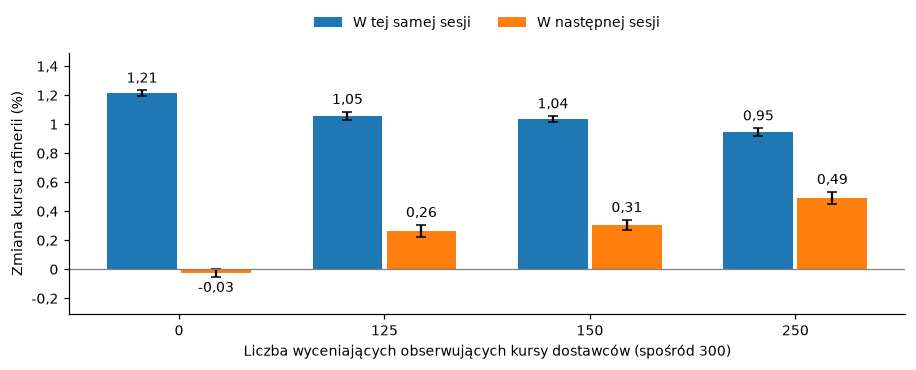
\includegraphics[width=0.94\textwidth]{f7_p7_network_share.png}
\caption{Reakcja kursów rafinerii na wzrost ich wyceny referencyjnej o~1\% w~czterech wariantach rynku.
Słupki przedstawiają średnie z~30 przebiegów, a~kreski --- przedziały 95\% z~5000 losowań bootstrapowych po ziarnach.}\label{fig:e7}
\end{figure}

Między skrajnymi wariantami oszacowana reakcja na wzrost wyceny referencyjnej o~1\% zmalała w~tej samej
sesji z~1,21\% do 0,95\%, a~w~następnej wzrosła z~$-0{,}03$\% do 0,49\% (rys.~\ref{fig:e7}).
Łączna odpowiedź w~dwóch sesjach wzrosła z~1,19\% do 1,44\%. Wzrost współczynnika reakcji w~następnej sesji
wyniósł 0,055 [0,047; 0,062] dla 18 spółek łącznie wobec 0,515 dla rafinerii.

\paragraph{Czy podobny wynik widać dla samej ropy?}
Porównaliśmy rzeczywiste i~symulowane stopy zwrotu VLO i~MPC w~tych samych 490 sesjach z~lat 2024--2025.
Dla każdej rafinerii zastosowaliśmy tę samą regresję dziennych stóp zwrotu na bieżące i~wczorajsze zmiany
wszystkich pięciu sygnałów zewnętrznych, po czym uśredniliśmy współczynniki obu spółek.

\begin{figure}[!htbp]
\centering
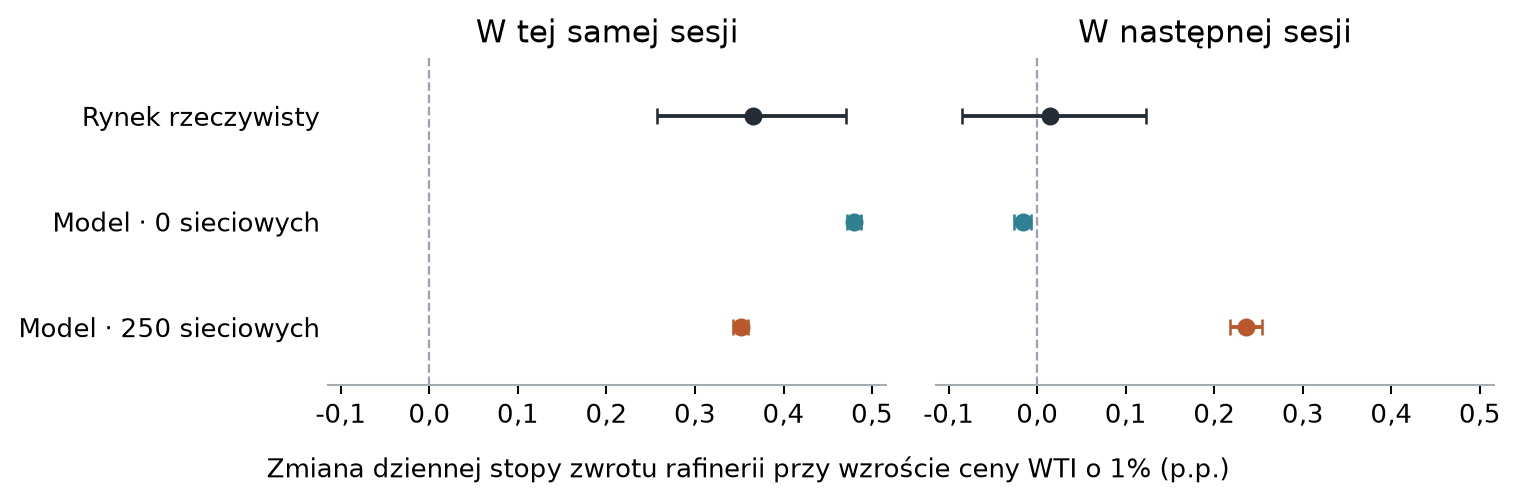
\includegraphics[width=\textwidth]{f7_p7_wti_refineries.png}
\caption{Oszacowana zmiana dziennej stopy zwrotu VLO i~MPC przy wzroście ceny WTI o~1\%, w~tej samej
i~w~następnej sesji. Punkty pokazują średnie oszacowania dla obu rafinerii. Przedziały 95\% obliczono
bootstrapem po blokach 10 kolejnych sesji dla rynku rzeczywistego oraz po 30 przebiegach na tej samej
historii cen dla każdego wariantu symulacji.}\label{fig:e7-wti}
\end{figure}

W~dniu wzrostu ceny WTI o~1\% oszacowana reakcja rzeczywistych rafinerii wyniosła $+0{,}37$~p.p.
W~wariancie z~250 wyceniającymi sieciowymi wyniosła $+0{,}35$~p.p., a~w~wariancie bez nich $+0{,}48$~p.p.
W~następnej sesji oszacowanie dla rynku było bliskie zeru ($+0{,}01$~p.p., przedział 95\% [$-0{,}09$;
$+0{,}12$]), podczas gdy w~symulacji wyniosło $+0{,}24$~p.p. przy 250 wyceniających sieciowych i~$-0{,}02$~p.p.
przy ich braku (rys.~\ref{fig:e7-wti}). Różnica między wariantami wyniosła 0,253~p.p. (95\% przedział
bootstrapowy [0,237; 0,269] dla 30 par przebiegów). Wariant sieciowy był więc bliższy oszacowaniu dla rynku
w~dniu zmiany ceny ropy, a~w~następnej sesji dawał silniejszą reakcję, niż wskazywały dane.

Jest to dodatkowe porównanie w~okresie użytym do kalibracji (rozdz.~\ref{sec:plan}). Decyzja w~sprawie H1
opiera się na zaplanowanym porównaniu reakcji rafinerii na zmianę ich wyceny referencyjnej (rys.~\ref{fig:e7}).

W~E1 źródło cen i~wagi zmieniają się razem, więc wynik dotyczy całej reguły wyceny. Wpływ źródła ceny można
sprawdzić, podając tym samym inwestorom sieciowym wartość referencyjną dostawcy $R_j$ w~miejsce jego kursu $P_j$,
przy tych samych wagach i~opóźnieniach obserwacji.

\clearpage
\subsection{P2. \questionTwo{} (E2)}\label{sec:p5}

Na tej samej historii cen surowców i~indeksu porównaliśmy trzy składy inwestorów przy trzech wagach
naśladowania ($h$).

Przejście do składu z~większym udziałem inwestorów trendowych i~zwiększenie wagi naśladowania podniosły wzmocnienie zmienności
($A_\sigma$), liczbę dużych odchyleń od wyceny referencyjnej ($N_{10}$) oraz reakcję w~następnej sesji
($\pi_1$). Zmiana z~\cell{mixed} na \cell{trend} bez naśladowania dała średnio o~118 przypadków dużego
odchylenia więcej na przebieg. Zwiększenie $h$ z~0 do 0,4 w~składzie \cell{mixed} dało ich o~30 więcej.

\begin{figure}[!htbp]
\centering
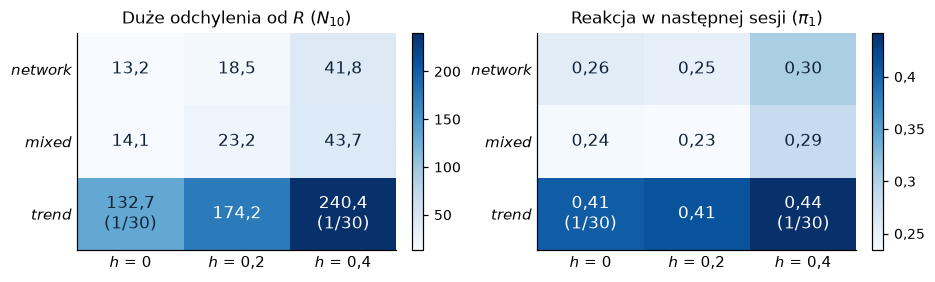
\includegraphics[width=\textwidth]{f7_e5_cells.png}
\caption{Średnia liczba dużych odchyleń od wyceny referencyjnej i~średnia reakcja w~następnej sesji dla każdego
składu i~wagi naśladowania. Średnie obejmują przebiegi bez załamania.
W~nawiasach podano liczbę załamań względem liczby przebiegów w~danym wariancie. Skale barw różnią się między panelami.}\label{fig:e5-cells}
\end{figure}

Na rysunku~\ref{fig:e5-cells} jeden przypadek dużego odchylenia oznacza jedną spółkę w~jednej sesji
z~$|\ln(P/R)|>0{,}1$. W~składzie \cell{trend} liczba takich przypadków rośnie wraz z~naśladowaniem
znacznie silniej niż w~\cell{mixed}. Reakcja w~następnej sesji jest natomiast wyższa w~\cell{trend}
już przy $h=0$. Tabela~\ref{tab:h3} pokazuje, jak duży jest efekt każdej z~tych zmian i~jak dokładnie go oszacowano.

\begin{table}[!htbp]
\centering\small
\caption{Zmiany trzech wskaźników E2 względem składu \cell{mixed} bez naśladowania.}\label{tab:h3}
\begin{tabular}{@{}l c c@{}}
\toprule
Wskaźnik & \makecell{Zmiana składu na \cell{trend}\\przy $h=0$}
         & \makecell{Zwiększenie $h$ do 0,4\\w~składzie \cell{mixed}} \\
\midrule
Wzmocnienie zmienności ($A_\sigma$) & $+0{,}193$ [0,177; 0,210] & $+0{,}102$ [0,088; 0,115] \\
Liczba dużych odchyleń ($N_{10}$) & $+118$ [90; 150] & $+30$ [22; 37] \\
Reakcja w~następnej sesji ($\pi_1$) & $+0{,}169$ [0,160; 0,177] & $+0{,}048$ [0,041; 0,055] \\
\bottomrule
\end{tabular}
\tablenote{Średnie różnice w~parach o~tym samym ziarnie i~przedziały bootstrapowe 95\% bez korekty.
Zmiana składu obejmuje 29 par, a~zmiana wagi naśladowania 30 par.}
\end{table}

Dla każdego z~trzech wskaźników kontrast \cell{trend} względem \cell{mixed} pozostaje dodatni przy każdej
wadze, a~kontrast $h=0{,}4$ względem $h=0$ pozostaje dodatni w~każdym składzie. Wszystkie te różnice
spełniają kryterium po poprawce Bonferroniego, więc potwierdzamy H2 (tab.~\ref{tab:reguly}).

Wyniki dotyczą całych reguł modelu. Wpływ strategii trendowej można sprawdzić, zmieniając jej udział przy
stałej proporcji obu typów wyceniających. Przy większym $h$ inwestor słabiej reaguje też na własną ocenę.
W~sprawdzeniu na jednym ziarnie sygnał znajomych był zerowy w~około dwóch trzecich decyzji, w~których
własny sygnał był niezerowy. Utrzymanie stałej wagi własnego sygnału pozwoliłoby oszacować wkład zleceń znajomych.

\FloatBarrier
\subsection{P3. \questionThree{} (E3a, E3b)}\label{sec:p6}

Na tej samej historii rynku włączaliśmy i~wyłączaliśmy limit ryzyka oraz rebalansowanie (E3a), a~przy stałych
cenach surowców i~indeksu porównaliśmy przebiegi z~wiadomością o~NVDA i~bez niej (E3b).

Po wyłączeniu obu reguł średnia korelacja reszt w~parach niepowiązanych ($\rho_u$) zmieniła się o~$-0{,}0009$
[$-0{,}0067$; 0,0052] bez naśladowania i~o~$-0{,}0003$ [$-0{,}0040$; 0,0038] przy $h=0{,}4$.
Odrzucamy H3 dla obu reguł (tab.~\ref{tab:reguly}). Po wiadomości o~NVDA największe spadki
odnotowaliśmy w~tej spółce i~u~jej dwóch sąsiadów w~grafie.

\begin{figure}[!htbp]
\centering
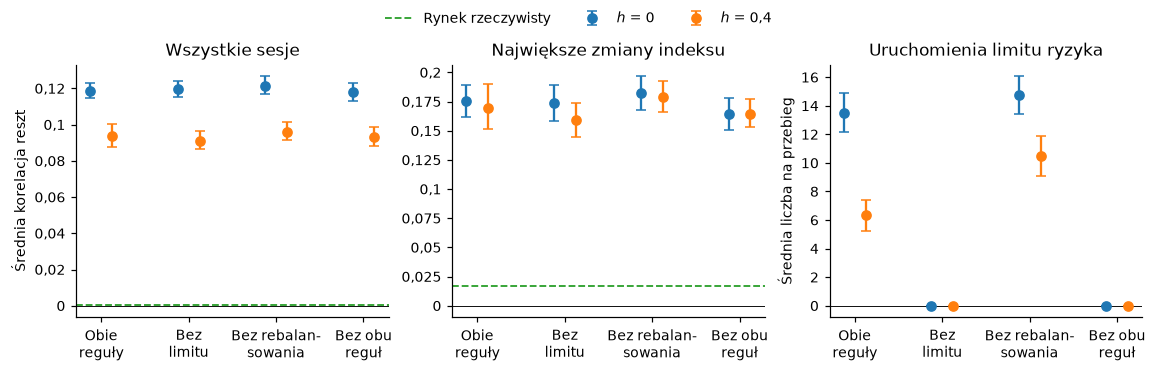
\includegraphics[width=\textwidth]{f7_p6_channels.png}
\caption{Skutki wyłączenia reguł portfelowych w~E3a. Dwa pierwsze panele pokazują średnią korelację reszt
w~całym okresie i~w~10\% sesji o~największych bezwzględnych zmianach indeksu. Linia przerywana oznacza
wynik dla tych samych par na rzeczywistym rynku. Prawy panel pokazuje średnią liczbę uruchomień limitu ryzyka
na przebieg. Odcinki oznaczają przedziały 95\%.}\label{fig:e6a}
\end{figure}

\paragraph{E3a.} Dla każdej z~109 par korelowaliśmy tę część dziennych stóp zwrotu, która pozostaje
po uwzględnieniu wyceny referencyjnej każdej spółki. Żaden wariant wyłączenia reguł nie dał wyraźnego
spadku korelacji, także w~sesjach o~największych ruchach indeksu. Przy obu regułach limit ryzyka
uruchamiał sprzedaż średnio 13,5 raza na przebieg bez naśladowania i~6,4 raza przy $h=0{,}4$.
Po wyłączeniu limitu takich uruchomień było zero (rys.~\ref{fig:e6a}).

\begin{figure}[!htbp]
\centering
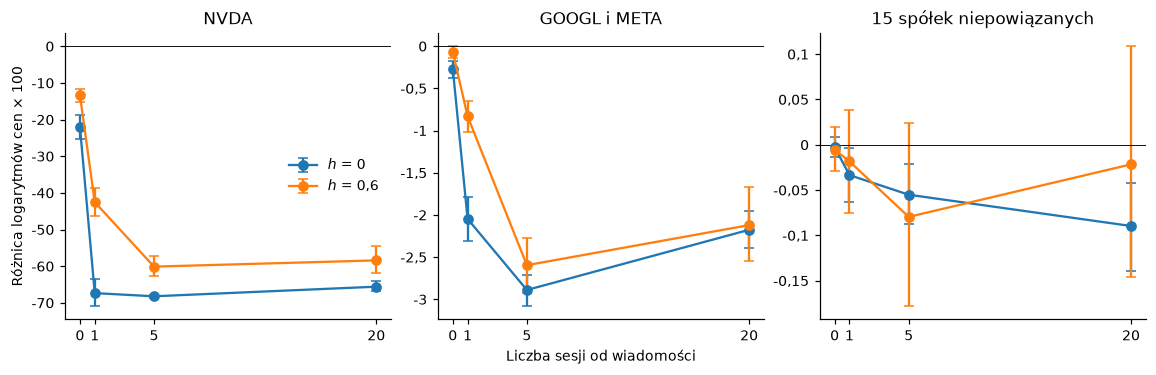
\includegraphics[width=\textwidth]{f7_p6_shock.png}
\caption{Wpływ wiadomości o~NVDA na kurs tej spółki, na kursy GOOGL i~META oraz na kursy pozostałych 15 spółek.
Punkty pokazują średnią różnicę logarytmów cen pomnożoną przez 100 (30 par przebiegów, przedziały 95\%).
Zero na osi poziomej oznacza zamknięcie sesji z~wiadomością. Każdy panel ma inną skalę pionową.}\label{fig:e6b}
\end{figure}

\paragraph{E3b.} Po obniżeniu wyceny NVDA o~połowę kurs tej spółki bez naśladowania odzwierciedlił
na zamknięciu około jednej trzeciej szoku w~skali logarytmicznej, a~na koniec następnej sesji prawie cały.
Po pięciu sesjach kursy GOOGL i~META były średnio o~około 2,9\% niższe niż w~przebiegach bez wiadomości.
Spadek pokazuje konsekwencję krawędzi od NVDA do tych spółek, które dodaliśmy ręcznie. W~pozostałych 15
spółkach średnia zmiana wyniosła $-0{,}06$ punktu logarytmicznego, a~średnia wielkość zmiany bez względu
na znak wyniosła 0,34 punktu. Część zmian poza sąsiedztwem NVDA znosiła się zatem w~średniej
(rys.~\ref{fig:e6b}).

\begin{samepage}
Inwestorzy nadal korzystali ze wspólnej gotówki, a~testowany kanał sprzedaży portfelowej miał ograniczony
zasięg, bo portfele obejmowały cztery spółki, a~limit ryzyka dotyczył 25\% inwestorów.\par
\end{samepage}

\subsection{Załamania przebiegów}

Poza E3b próg załamania przekroczyły dwa z~570 przebiegów, oba w~składzie \cell{trend} w~E2.
Ponowne obliczenie głównych porównań E2 z~uwzględnieniem obu przebiegów daje tę samą decyzję dla H2
(dodatek~\ref{sec:zal-osobno}).

\section{Walidacja: co model odtwarza, a~czego nie}\label{sec:walidacja}

Wyniki E1--E3 opisują reakcje wewnątrz symulacji. Poniżej sprawdzamy, na ile przypominają one reakcje na rzeczywistym rynku
i~ile do tego dopasowania wnosi graf. Wagi z~lat 2021--2023 sprawdzamy na stopach zwrotu z~lat 2024--2025
(rozdz.~\ref{sec:poza-proba}). Trajektoria $R$ korzysta tu z~cen surowców i~indeksu z~tej samej sesji.
Następnie sprawdzamy, czy jednodniowe opóźnienia widoczne w~symulacji wykrywamy również na rzeczywistym rynku
(rozdz.~\ref{sec:opoznienia}).
Porównania przebiegów rynku agentowego z~danymi dotyczą okresu użytego do kalibracji (rozdz.~\ref{sec:plan}).
Ponieważ te same własności statystyczne odtwarza wiele modeli~\cite{fagiolo2007}, każde
porównanie ma kontrolę, bez której nie da się go zinterpretować:
\begin{itemize}
  \item dla wartości liczonych z~$R$: $R$ 200 grafów losowych, czyli krawędzi badanego grafu z~losowo zamienionymi
  rodzicami i~dziećmi (każda spółka zachowuje liczbę rodziców, każdy rodzic --- liczbę dzieci) i~wagami
  oszacowanymi na nowo na latach 2021--2023;
  \item dla symulacji: komórka główna (\cell{mixed}, $h = 0{,}2$) na dwóch grafach losowych i~na płaskich wejściach
  (stałe sygnały zewnętrzne), na 10 ziarnach wspólnych z~komórką główną.
\end{itemize}
Zgodność wyniku z~kontrolą ogranicza możliwość przypisania go badanemu mechanizmowi.

\subsection{Graf poza próbą}\label{sec:poza-proba}

\begin{figure}[!htbp]
\centering
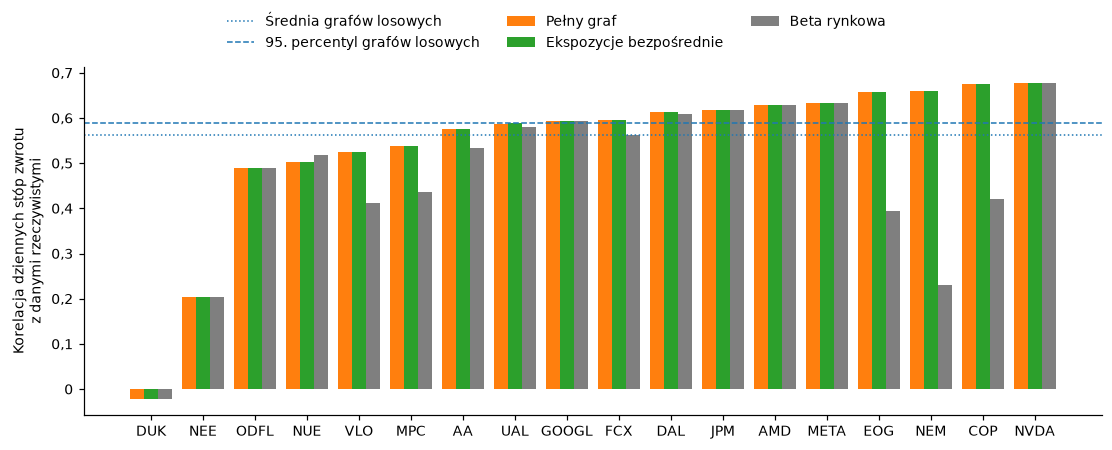
\includegraphics[width=\textwidth]{f8_out_of_sample.png}
\caption{Korelacja dziennej stopy zwrotu $R$ (wagi 2021--2023, prawdziwe sygnały 2024--2025) z~prawdziwą stopą
zwrotu każdej spółki w~latach 2024--2025, obok $R$ z~samymi bezpośrednimi ekspozycjami (bez krawędzi między
spółkami) i~samej bety rynkowej. Linie: średnia i~95.~percentyl dla 200 grafów losowych.}\label{fig:oos}
\end{figure}

Mediana po spółkach korelacji $R$ z~prawdziwą stopą zwrotu wynosi 0,595, a~samej bety rynkowej 0,526
(rys.~\ref{fig:oos}). Grafy
losowe dają średnio 0,563 (95.~percentyl 0,590) i~żaden z~200 nie osiąga mediany badanego grafu. Taką samą medianę,
0,595, daje jednak $R$ z~samymi bezpośrednimi ekspozycjami spółek na surowce i~indeks, bez krawędzi między
spółkami. Dla poszczególnych spółek różnice były rzędu jednej tysięcznej lub mniejsze. Przewagę nad grafami losowymi daje więc
właściwy dobór ekspozycji na surowce (grafy losowe przestawiają także krawędzie surowiec $\to$ spółka), a~nie
krawędzie między spółkami. Wagi bezpośrednie są szacowane na tych samych danych i~mogą ujmować łączne ekspozycje związane z~kilkoma ścieżkami (rozdz.~\ref{sec:graf}). Krawędzie między spółkami mają znaczenie wewnątrz modelu, bo od nich
zależy, kiedy reagują wyceniający sieciowi (rozdz.~\ref{sec:p7}), ale ich dodatkowej wartości dla objaśnienia
prawdziwego rynku ten sprawdzian nie pokazuje. Graf zyskuje na spółkach surowcowych (COP 0,67 wobec 0,42 dla bety, EOG 0,66 wobec 0,40, NEM 0,66 wobec 0,23, VLO 0,53 wobec
0,41). Dla spółek technologicznych i~JPM $R$ zawiera tylko ruch indeksu, więc równa się becie. Dla DUK korelacja
jest bliska zeru w~obu modelach ($-0{,}02$): w~latach 2024--2025 ta spółka energetyczna nie podążała ani za
indeksem, ani za gazem.

\subsection{Przewidywalne opóźnienia}\label{sec:opoznienia}
W~E1 mierzyliśmy, jak kursy dwóch rafinerii reagują na zmianę ich własnej wyceny referencyjnej w~tej samej
i~w~następnej sesji (rozdz.~\ref{sec:p7}). Dla tych samych rafinerii zestawiliśmy też symulowaną i~rzeczywistą
reakcję na WTI (rys.~\ref{fig:e7-wti}). Tutaj sprawdzamy, czy wczorajsza stopa zwrotu rodzica pozwala przewidzieć
dzisiejszą stopę zwrotu dziecka na danej krawędzi, zarówno w~symulacji, jak i~w~danych rzeczywistych.
Test obejmuje 29 krawędzi z~pominięciem indeksu (15 surowiec--spółka i~14 spółka--spółka). Dla surowców
zmienną objaśniającą jest w~obu porównaniach wczorajsza historyczna stopa zwrotu.

\begin{table}[!htbp]
\centering\small
\caption{Opóźnienie o~jedną sesję: udział testów z~$|t| > 2$.}\label{tab:lag}
\begin{tabular}{@{}l c c@{}}
\toprule
 & udział testów z~$|t| > 2$ & mediana $t$ \\
\midrule
prawdziwe 2024--2025 & 0\% & $-0{,}36$ \\
symulacja, komórka główna & 62\% & 2,93 \\
symulacje na grafach losowych & 49\% i~45\% & --- \\
płaskie wejścia & 10\% & --- \\
\bottomrule
\end{tabular}
\end{table}

W~komórce głównej próg $|t|>2$ przekroczyło około 62\% testów liczonych dla 29 krawędzi w~każdym
z~30 przebiegów (tab.~\ref{tab:lag}). W~danych rzeczywistych próg nie został przekroczony w~żadnym z~29 testów.
W~tej próbie nie wykryliśmy więc jednodniowego opóźnienia. Cohen i~Frazzini~\cite{cohen} wykryli opóźnienia
między dostawcami a~odbiorcami w~danych miesięcznych.

\subsection{Reakcja na duże ruchy surowców}

\begin{figure}[!htbp]
\centering
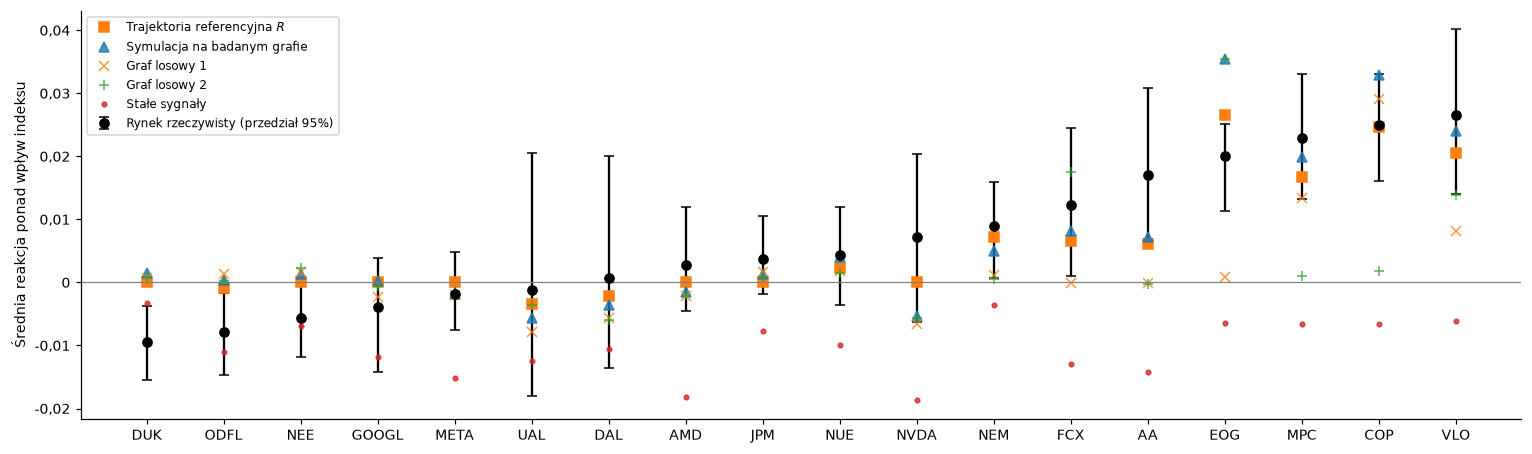
\includegraphics[width=\textwidth]{f8_event_study.png}
\caption{Dni 5\% największych ruchów ropy: średnia reakcja każdej spółki ponad betę rynkową, ze znakiem ruchu ropy.
Czarne punkty przedstawiają reakcje rzeczywiste. Przedziały 95\% uzyskano z~2000 losowań dziesięciosesyjnych bloków dat zdarzeń.}\label{fig:events}
\end{figure}

\begin{table}[!htbp]
\centering\small
\caption{Korelacja między spółkami średniej reakcji modelu i~prawdziwej reakcji w~dniach dużych ruchów surowca.}
\label{tab:events}
\begin{tabular}{@{}l c c c c c c@{}}
\toprule
 & \multicolumn{3}{c}{Trajektoria $R$} & \multicolumn{3}{c}{Symulacja} \\
\cmidrule(lr){2-4}\cmidrule(lr){5-7}
Zdarzenia & \makecell{badany\\graf} & \makecell{tylko\\bezpośr.} & \makecell{grafy\\losowe} & \makecell{badany\\graf}
  & \makecell{grafy\\losowe} & \makecell{płaskie\\wejścia} \\
\midrule
ropa, 1 dzień & 0,87 & 0,87 & 0,76 (15,5\%) & 0,82 & 0,61 / 0,48 & 0,19 \\ \addlinespace[2pt]
ropa, 2 dni & 0,84 & 0,84 & 0,67 (0,5\%) & 0,80 & 0,70 / 0,44 & 0,37 \\ \addlinespace[2pt]
miedź, 2 dni & 0,79 & 0,79 & 0,15 (0\%) & 0,75 & $-0{,}07$ / $-0{,}19$ & $-0{,}04$ \\
\bottomrule
\end{tabular}
\tablenote{$R$ grafów losowych: średnia z~200 grafów, w~nawiasie odsetek grafów z~wynikiem co najmniej takim jak
dla badanego grafu. Symulacja na grafach losowych: dwa grafy.}
\end{table}

Dla każdego surowca i~horyzontu wybrano 24 daty po rozgrzewce, według malejącej bezwzględnej zmiany ceny. Okna dwusesyjne nie nakładają się. Od stóp zwrotu odejmujemy iloczyn bieżącej stopy zwrotu indeksu i~bety oszacowanej przed 2024~r., sumujemy odpowiedź w~oknie i~orientujemy ją według znaku ruchu surowca. Model odtwarza, które spółki reagują na surowce i~jak mocno (tab.~\ref{tab:events}); stosunek wielkości reakcji
do prawdziwej wynosi 0,93 dla ropy w~1 dzień i~1,19 w~2 dni. Przewaga nad grafami losowymi jest wyraźna dla
miedzi i~dla dwudniowej reakcji na ropę; dla ropy w~1 dzień 15,5\% grafów losowych daje $R$ co najmniej tak dobre
jak badany graf. $R$ z~samymi bezpośrednimi ekspozycjami daje te same korelacje (0,8748 wobec 0,8745 dla ropy
w~1 dzień), więc i~tu dopasowanie pochodzi z~ekspozycji na surowce. W~jednodniowym porównaniu dla ropy znak
średniej reakcji zgadzał się z~danymi dla 11 z~18 spółek (61\%) w~symulacji i~dla 16 z~18 (89\%) w~trajektorii $R$.

\subsection{Własności statystyczne stóp zwrotu}

\begin{table}[!htbp]
\centering\small
\caption{Własności statystyczne dziennych stóp zwrotu.}\label{tab:facts}
\begin{tabularx}{\textwidth}{@{}Y c c c c@{}}
\toprule
 & prawdziwe 2024--2025 & $R$ & symulacja & płaskie wejścia \\
\midrule
autokorelacja $r$, opóźnienie 1 & $-0{,}035$ & $-0{,}060$ & 0,016 & $-0{,}524$ \\ \addlinespace[3pt]
autokorelacja $|r|$, opóźnienie 1 & 0,097 & 0,228 & 0,156 & 0,317 \\ \addlinespace[3pt]
kurtoza nadwyżkowa & 6,9 & 15,6 & 5,8 & 1,1 \\ \addlinespace[3pt]
odchylenie dzienne, \% & 2,27 & 1,29 & 1,72 & 0,63 \\ \addlinespace[3pt]
korelacja $\ln$ wolumenu z~$|r|$ & 0,50 & --- & 0,46 & 0,39 \\ \addlinespace[3pt]
korelacja z~prawdziwą stopą zwrotu & 1 & 0,595 & 0,456 & $-0{,}002$ \\
\bottomrule
\end{tabularx}
\end{table}

Symulacja ma grube ogony, grupowanie zmienności i~związek wolumenu z~wielkością ruchu bliskie rzeczywistym
(tab.~\ref{tab:facts}; por.~\cite{cont2001}). Te same własności dają jednak symulacje na grafach losowych (kurtoza 5,6 i~5,8), więc nie
sprawdzają grafu: pochodzą z~prawdziwych sygnałów i~z~mechaniki rynku. Na płaskich wejściach kurtoza spada do 1,1,
a~autokorelacja $-0{,}52$ to odbijanie ceny między stronami arkusza.

\paragraph{Przebieg kursów w~czasie.}
Podobne własności dziennych zwrotów mogą występować przy różnych trajektoriach cen. Dla każdej sesji wyznaczyliśmy
pasmo obejmujące środkowe 90\% symulowanych kursów zamknięcia przy tej samej historii sygnałów. W~zależności
od spółki mediana szerokości pasma wynosiła od około 2 do 5\% jego dolnej granicy. Kurs rzeczywisty mieścił
się w~paśmie w~zaledwie 0--9\% sesji. VLO, jedna z~rafinerii badanych w~E1, należy do spółek o~największej
zgodności (8,7\% sesji, rys.~\ref{fig:bands}). Na koniec okresu wszystkie rzeczywiste kursy były poza pasmem.
Zmiana ziaren daje więc niewielki rozrzut ścieżek cen przy zadanych cenach surowców i~indeksu.

\begin{figure}[!htbp]
\centering
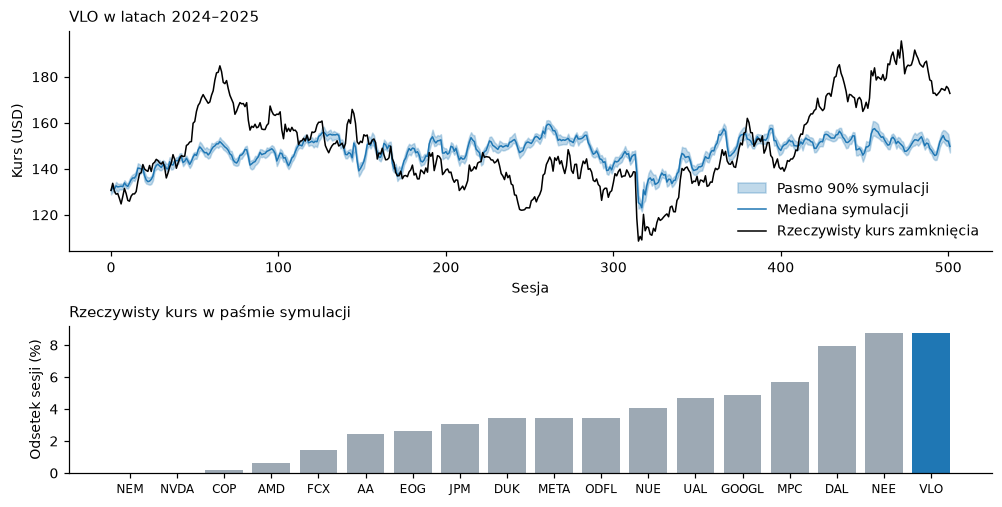
\includegraphics[width=\textwidth]{f8_bands.png}
\caption{Zgodność ścieżek cen z~rzeczywistymi kursami. U~góry kurs VLO przeskalowany do ceny startowej
symulacji, mediana i~pasmo od 5. do 95. percentyla przebiegów wariantu bazowego.
U~dołu odsetek sesji po rozgrzewce, w~których kurs rzeczywisty mieścił się w~paśmie, dla wszystkich
18 spółek. VLO wyróżniono kolorem.}\label{fig:bands}
\end{figure}

\FloatBarrier
\subsection{Odtwarzalność wag przy zadanej strukturze grafu}

\begin{figure}[!htbp]
\centering
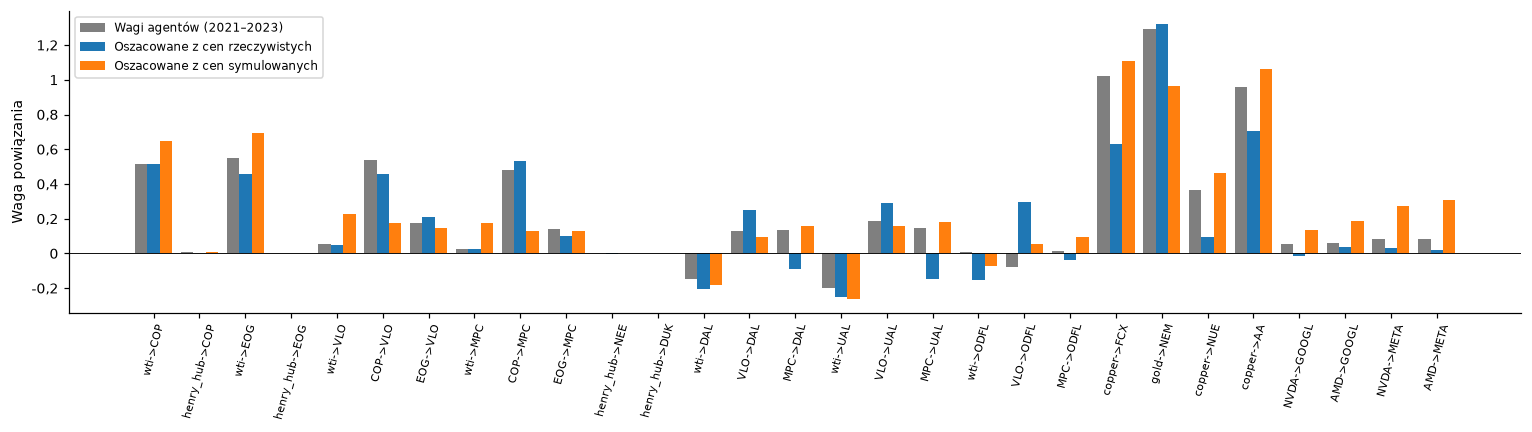
\includegraphics[width=\textwidth]{f8_graph_recovery.png}
\caption{Wagi powiązań między aktywami oszacowane na nowo tą samą regresją: z~prawdziwych cen 2024--2025 i~z~cen
symulowanych (średnia z~przebiegów komórki głównej), obok wag, których używają agenci.}\label{fig:recovery}
\end{figure}

Korelacja wag odbudowanych z~wagami agentów wynosi 0,88 dla symulacji, 0,91 dla prawdziwych cen 2024--2025, 0,23
i~0,31 dla symulacji na grafach losowych oraz $-0{,}04$ dla płaskich wejść. Wśród zadanych krawędzi 69\% w~symulacji i~41\% w~danych rzeczywistych ma ponownie
ten sam znak przy $|t|>2$. Test dotyczy wag przy ustalonych rodzicach każdej spółki.

\FloatBarrier
\subsection{Struktura korelacji}\label{sec:korelacje}

\begin{figure}[!htbp]
\centering
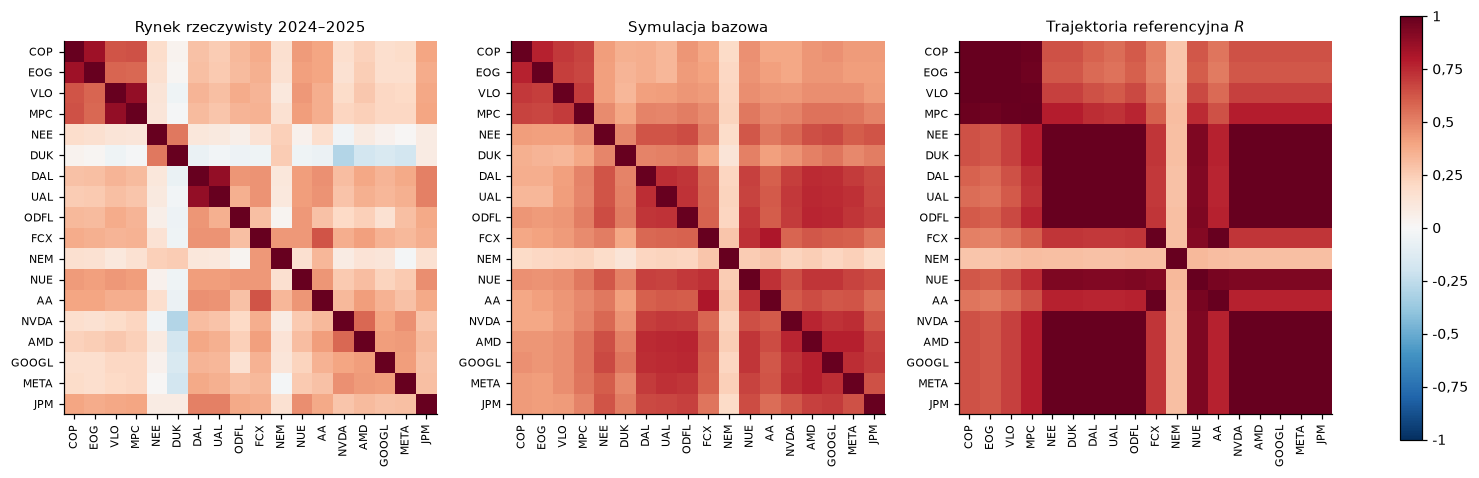
\includegraphics[width=\textwidth]{f8_correlation.png}
\caption{Korelacje dziennych stóp zwrotu 18 spółek: prawdziwe, w~symulacji (średnia z~przebiegów komórki głównej)
i~w~$R$.}\label{fig:corr}
\end{figure}

Wzór korelacji symulacja odtwarza lepiej niż $R$: korelacja 153 elementów macierzy symulowanej z~prawdziwą wynosi
0,42, dla $R$ --- 0,17, dla symulacji na grafach losowych --- 0,27 i~0,25. Poziom korelacji jest jednak za wysoki:
średnio 0,53 wobec 0,27 w~rzeczywistości ($R$: 0,76).

\begin{table}[!htbp]
\centering\small
\caption{Korelacja reszt: rynek prawdziwy i~symulowany.}
\label{tab:wspolruch}
\begin{tabularx}{\textwidth}{@{}Y c c c c@{}}
\toprule
Seria & \makecell{$\rho_u$ (pary\\niepowiązane)} & \makecell{udział par\\z~korelacją $> 0{,}1$} &
  \makecell{$\rho_u^{\mathrm{s}}$\\(dni stresu)} & \makecell{pary\\powiązane} \\
\midrule
prawdziwe spółki 2024--2025 & 0,000 & 0,31 & 0,017 & 0,191 \\ \addlinespace[3pt]
symulacja, komórka główna (\cell{mixed}, $h = 0{,}2$) & 0,121 & 0,54 & 0,200 & 0,136 \\ \addlinespace[3pt]
symulacja, płaskie wejścia (te same ziarna) & 0,002 & 0,03 & $-0{,}004$ & 0,001 \\
\bottomrule
\end{tabularx}
\end{table}

W~symulacji średnia korelacja reszt dla par niepowiązanych jest wyższa niż na rzeczywistym rynku
(0,121 wobec 0,000). Próg 0,1 przekracza 54\% par w~symulacji i~31\% na rynku. Przy stałych cenach
surowców i~indeksu średnia w~symulacji wynosi 0,002 (tab.~\ref{tab:wspolruch}). Jednym z~możliwych
wyjaśnień jest opóźniona reakcja wielu spółek na ruch indeksu, która mogłaby pozostać w~resztach mimo
uwzględnienia wyceny referencyjnej. Osobno nie testowaliśmy tego mechanizmu.

\FloatBarrier
\section{Dyskusja i~ograniczenia}\label{sec:dyskusja}\label{sec:ograniczenia}
Podobna zgodność dziennych stóp zwrotu z~danymi może towarzyszyć różnej dynamice dostosowania. W~E1 pełne wagi
przenoszą część ekspozycji VLO na ropę na kursy COP i~EOG. Taki mechanizm jest zgodny z~rolą ograniczonej uwagi
w~relacjach klient--dostawca~\cite{cohen,menzly2010}. Wynik E1 dotyczy dwóch rafinerii i~sieci zbudowanej na
podstawie powiązań branżowych. W~sprawdzianie obejmującym wszystkie 29 krawędzi z~pominięciem indeksu
jednodniowe opóźnienie wykryliśmy znacznie częściej w~symulacji niż w~danych (rozdz.~\ref{sec:opoznienia}).
Skalę tej rozbieżności można sprawdzić w~innym okresie przy niezmienionych parametrach.

Zmiany składu i~siły naśladowania w~E2 pokazują, jak szeroko kursy mogą odchodzić od tej samej wyceny
referencyjnej.

W~wariancie bazowym średnia korelacja reszt w~parach niepowiązanych wynosiła 0,121, a~na rzeczywistym
rynku była bliska zeru (tab.~\ref{tab:wspolruch}). W~E3a po jednoczesnym wyłączeniu limitu ryzyka
i~rebalansowania oszacowana zmiana tej korelacji była mniejsza niż 0,001 co do wartości bezwzględnej przy obu
badanych poziomach naśladowania (rozdz.~\ref{sec:p6}).
Model wytwarza zatem nadmierny współruch, a~dwie badane reguły portfelowe mają w~tych wariantach niewielki
wpływ na jego wielkość. We wszystkich wariantach E3a inwestorzy finansowali zakupy różnych akcji z~tego samego
salda gotówki. Wkład tego mechanizmu pozostaje otwarty. Można go ocenić, porównując wspólne saldo z~osobnym
saldem dla każdej akcji.

\section{Wnioski}
Większy udział wyceniających sieciowych osłabił reakcję rafinerii w~dniu zmiany wyceny referencyjnej i~wzmocnił ją
w~następnej sesji oraz w~obu sesjach łącznie (P1). W~porównaniu reakcji na WTI wariant sieciowy był bliższy
oszacowaniu dla rzeczywistych rafinerii w~dniu zmiany ceny ropy, a~w~następnej sesji dawał silniejszą reakcję.

Skład z~większym udziałem inwestorów trendowych oraz silniejsze naśladowanie zwiększyły zmienność, odchylenia
od wyceny referencyjnej i~reakcję w~następnej sesji (P2). Po wyłączeniu limitu ryzyka i~rebalansowania
współruch spółek niepowiązanych pozostał zbliżony, a~wspólne saldo gotówki działało we wszystkich wariantach E3a (P3).

Oba warianty wyceny referencyjnej, z~pełnym grafem i~z~bezpośrednimi ekspozycjami, osiągnęły podobną zgodność
z~dziennymi stopami zwrotu spółek. Jednocześnie w~symulacji wczorajsze zmiany cen dostawców i~surowców znacznie
częściej wiązały się z~dzisiejszymi zmianami cen ich odbiorców niż w~danych z~lat 2024--2025.

Rolę ceny dostawcy w~tym opóźnieniu można sprawdzić, porównując reakcję rafinerii przy tych samych wagach
i~opóźnieniach obserwacji, gdy inwestorzy korzystają z~symulowanego kursu dostawcy albo z~jego wyceny
referencyjnej. Dane z~niezależnego okresu pozwolą ocenić, czy rozbieżność w~tempie dostosowania utrzymuje
się poza badaną próbką.

\paragraph{Dostępność kodu i~danych.}
Kod i~instrukcja odtworzenia analiz są w~\href{https://github.com/dmitrykitty/stock-exchange-simulation}{repozytorium projektu}.
Do raportu dołączono archiwum tabel z~pełnymi kontrastami i~wynikami walidacji, a~źródła danych podano
w~tabeli~\ref{tab:dane}.

\clearpage
\appendix
\section{Pilotaż i~odstępstwa od projektu}\label{sec:odstepstwa}
W~protokole badania i~w~repozytorium eksperymenty, pytania i~hipotezy mają numerację wniosku badawczego, w~którym
były też eksperymenty pilotażowe na rynkach uproszczonych. Tabela~\ref{tab:numeracja} podaje odpowiedniki.

\begin{table}[!htbp]
\centering\small
\caption{Numeracja w~artykule i~w~protokole badania.}\label{tab:numeracja}
\begin{tabular}{@{}l l l l@{}}
\toprule
Artykuł & Protokół i~repozytorium & Pytanie & Hipoteza \\
\midrule
E1 & E7 & P1 = P7 & H1 = H5 \\
E2 & E5 & P2 = P5 & H2 = H3 \\
E3a, E3b & E6a (kanały), E6b (wiadomość o~spółce) & P3 = P6 & H3 = H4 \\
\bottomrule
\end{tabular}
\end{table}

\begin{table}[!htbp]
\centering\small
\caption{Odstępstwa badania głównego od wniosku badawczego.}\label{tab:odstepstwa}
\begin{tabularx}{\textwidth}{@{}Y Y Y@{}}
\toprule
Wniosek & Badanie główne & Dlaczego \\
\midrule
ok.~1000 agentów & 525 inwestorów i~36 animatorów & czas przebiegu; na spółkę przypada ok.~110 inwestorów \\ \addlinespace[3pt]
„kupuj, dopóki sygnał dodatni” & pozycja docelowa & stara reguła dawała autokorelację stóp zwrotu $+0{,}59$ \\ \addlinespace[3pt]
limit ryzyka u~wszystkich & u~25\% inwestorów & limit u~wszystkich wywoływał spiralę sprzedaży i~krach \\ \addlinespace[3pt]
animator centruje kwotowania na midpoincie z~własnymi kwotowaniami & na midpoincie bez własnych kwotowań & dawny
  przesuw za zapas sumował się przy każdym przebudzeniu; w~pilotażu usuwa 4 z~6 załamań bez zmiany kalibracji
  komórki głównej \\ \addlinespace[3pt]
eksperyment z~portfelem wspólnym i~rozdzielonym & E3a (wyłączniki kanałów) i~E3b (wiadomość o~spółce) &
  rozdz.~\ref{sec:eksperymenty} \\ \addlinespace[3pt]
współruch $\operatorname{corr}(r^P) - \operatorname{corr}(r^R)$ & korelacja reszt $\rho_u$ &
  rozdz.~\ref{sec:miary} \\ \addlinespace[3pt]
eksperymenty na rynkach uproszczonych w~badaniu głównym & etapy wstępne, niepowtarzane & uproszczone rynki
  (1 aktywo, łańcuch 3 spółek); eksperyment na łańcuchu sprawdzony z~nową regułą animatora: wnioski bez zmian \\
\bottomrule
\end{tabularx}
\end{table}

\FloatBarrier
\subsection{Weryfikacja implementacji}\label{sec:impl}
Testy kontraktowe obejmują priorytet ceny i~czasu oraz rozliczanie częściowych wykonań. Losowe sekwencje
zleceń porównują implementacje Python i~C++. Metadane wszystkich 690 przebiegów wykazują zgodność początkowych
i~końcowych sum gotówki i~liczb akcji według aktywów. Powtarzalność sprawdza się dla jednakowej konfiguracji i~ziarna.
Wersje repozytorium zapisane w~metadanych przebiegów mają te same moduły symulacji i~konfiguracje badania.

\FloatBarrier
\section{Załamania i~sprawdzenie wrażliwości}\label{sec:zal-osobno}

W~E2 po jednym załamaniu wystąpiło w~składzie \cell{trend} przy $h=0$ i~$h=0{,}4$. W~każdym z~tych
wariantów było to 1 na 30 przebiegów (95\% przedział Wilsona [0,006; 0,167]). Kurs DAL spadł do 17,85~USD
przy wycenie referencyjnej 47,97~USD. Akcjami AMD handlowano po 1--2 centy przy wycenie 179,61~USD
(63 transakcje w~sesji). Oba zdarzenia zaczęły się w~sesjach 318--320, podczas spadków z~kwietnia 2025~r.
W~wariantach \cell{trend} z~$h>0$ załamał się 1 z~60 przebiegów, a~w~pozostałych wariantach E2
1 z~210 (jednostronny test Fishera, $p=0{,}40$). W~pilotażu, przed zmianą reguły animatora, w~składzie
\cell{trend} przy $h\geq 0{,}2$ próg przekroczyło 6 z~60 przebiegów.

W~analizie wrażliwości przywróciliśmy oba przebiegi do porównań parowych E2 i~zastosowaliśmy tę samą
regułę statystyczną. Wszystkie 18 głównych różnic pozostało dodatnich po poprawce Bonferroniego.
Przykładowo zmiana z~\cell{mixed} na \cell{trend} przy $h=0$ zwiększyła liczbę dużych odchyleń
średnio o~120 zamiast 118 na przebieg.

\begin{samepage}
W~E3b próg przekroczyły 32 z~60 przebiegów z~wiadomością (23 przy $h=0$ i~9 przy $h=0{,}6$).
Wiadomość obniża wycenę NVDA o~połowę, podczas gdy $R$ pozostaje na wcześniejszym poziomie.
Dlatego w~E3b próg służy wyłącznie do opisu odchylenia, zgodnie z~regułą z~rozdziału~\ref{sec:miary}.\par
\end{samepage}

\clearpage
\section{Oznaczenia}\label{sec:oznaczenia}

\begin{table}[!ht]
\centering\small
\caption{Oznaczenia używane w~równaniach.}\label{tab:oznaczenia}
\begin{tabular}{@{}l >{\raggedright\arraybackslash}p{0.72\textwidth}@{}}
\toprule
Symbol & Znaczenie \\
\midrule
\multicolumn{2}{@{}l}{\textit{Graf zależności}} \\ \addlinespace[2pt]
$r_{i,t}$ & dzienna logarytmiczna stopa zwrotu spółki $i$ w~dniu $t$ \\
$\mathcal P_i$ & rodzice spółki $i$ w~grafie: sygnały zewnętrzne, indeks i~--- w~wagach pełnych --- spółki-dostawcy \\
$w_{ij}$ & waga krawędzi $j \to i$: o~ile procent zmienia się wycena spółki $i$, gdy rodzic $j$ zmienia się o~1\% \\
$\beta_i$, $r^{\mathrm{S\&P500}}_t$ & wrażliwość spółki na rynek i~dzienna stopa zwrotu indeksu \\
$\alpha_i$, $u_{i,t}$ & wyraz wolny i~reszta regresji \\
\cmidrule(lr){1-2}
\multicolumn{2}{@{}l}{\textit{Wycena i~sygnał inwestora}} \\ \addlinespace[2pt]
$V_{a,i}(t)$ & wycena spółki $i$ przez agenta $a$ w~chwili $t$; $V_{a,i}(0)$ to cena startowa z~osobistym błędem
  agenta (odchylenie standardowe 2\%) \\
$P_i(t)$ & cena spółki na symulowanej giełdzie; dla sygnału zewnętrznego --- jego poziom z~danych \\
$P^{\mathrm{obs}}_{a,j}(t)$ & cena rodzica widziana przez agenta z~opóźnieniem: $P_j(t - d_a)$, średnio $d_a = 0{,}05$
  sesji \\
$\hat w_{a,ij}$ & waga z~osobistym błędem agenta: $w_{ij}(1 + \eta_{a,ij})$, $\sigma_\eta = 0{,}1$ \\
$b$, $\gamma$ & sygnał własny agenta w~przedziale $[-1, 1]$; odchylenie wyceny od ceny, przy którym sygnał osiąga
  $\pm 1$ ($\gamma = 0{,}05$) \\
$s$, $h$, $\bar d$ & sygnał końcowy, siła naśladowania i~średni kierunek ostatnich zleceń znajomych \\
\cmidrule(lr){1-2}
\multicolumn{2}{@{}l}{\textit{Trajektoria referencyjna}} \\ \addlinespace[2pt]
$R_i(t)$ & cena referencyjna spółki $i$ w~sesji $t$; $R_i(0)$ to cena startowa \\
$X_k(t)$ & poziom sygnału zewnętrznego $k$ (ropa, gaz, miedź, złoto, indeks) z~danych \\
\cmidrule(lr){1-2}
\multicolumn{2}{@{}l}{\textit{Wskaźniki}} \\ \addlinespace[2pt]
$P_{i,t}$, $R_{i,t}$ & cena spółki i~jej trajektoria referencyjna na koniec sesji $t$ \\
$r^P_{i,t}$, $r^R_{i,t}$ & dzienne stopy zwrotu ceny i~trajektorii referencyjnej \\
$\pi_0$, $\pi_1$ & reakcja ceny na zmianę $R$ w~tej samej i~następnej sesji; $\pi^{(2)}_0$,
  $\pi^{(2)}_1$ --- to samo dla rafinerii \\
$\Pi^{(2)}$ & łączna odpowiedź rafinerii w~dwóch sesjach: $\pi^{(2)}_0 + \pi^{(2)}_1$ \\
$A_\sigma$ & wzmocnienie zmienności: mediana po spółkach stosunku $\sigma(\Delta \ln P)$ do $\sigma(\Delta \ln R)$ \\
$N_{10}$ & liczba spółko-dni z~$|\ln (P/R)| > 0{,}1$ \\
$u_{i,t}$ & reszta stopy zwrotu po usunięciu części wyjaśnionej przez własne $R$ spółki \\
$\rho_u$, $\rho_u^{\mathrm{s}}$ & średnia korelacja reszt par niepowiązanych: we wszystkie dni i~w~dniach stresu \\
$\Delta_{i,k}$ & różnica $\ln P$ spółki $i$ z~wiadomością i~bez niej $k$ sesji po wiadomości \\
\bottomrule
\end{tabular}
\end{table}

% =================================================================================================================
\bibliographystyle{unsrtnat}
\bibliography{references}

\end{document}
